\cleardoublepage%
\chapter{\label{chap:first}The Standard Model of Particle Physics}%
\noindent The Standard Model (SM) of particle physics describes the theoretical framework in which the work of this thesis is interpreted. In Section \ref{subsec:SM_particles} a brief overview of the particles of the SM is given. The interactions and properties of these particles are described by gauge theories which are discussed in Section \ref{sec:intro_gauge}. In particular, in Section \ref{sec: QED}, a brief overview of Quantum Electrodynamics is presented followed by the description of Quantum Chromodynamics in Section \ref{intro_QCD}. The discussion continues with the electroweak unification, an important aspect of the SM, in Section \ref{subsec:Electroweak}.  Based on these discussions, an open question of the SM is the origin of particle masses, which will be discussed in Section \ref{sec:intro_symmetry}. In Sections \ref{intro_top} and \ref{intro_Higgs} a quick overview of the top quark and the Higgs boson is presented respectively followed by the associated production of these two particles in Section \ref{intro_ttH}. Finally, in Section \ref{intro_ttbb} the production of top quark-antiquark pairs with the addition of emitted jets is emphasized, the main subject of this thesis.\\
\indent All discussions and results in this thesis are presented using natural units, following the convention $c = \hbar = 1$. To this effect, energies, momenta and masses all have units of energy, commonly expressed in electronvolt, $1 eV = 1.6\cdot 10^{-19} J$. Similarly, electric charge is given in elementary units, $1e = 1.6\cdot 10^{-19} C$. Additionally, throughout this thesis, Einstein's convention of summation over repeated indices is employed.

%\section{\label{sec:SM}The Standard Model}%
% \indent The Standard Model (SM) provides the modern understanding of all of the interactions of subatomic particles, except those due to gravity. The theory has emerged as the best distillation of decades of research and represents one of the triumphs of modern physics. With the discovery of the Higgs boson at the Large Hadron Collider, all of particles in the Standard Model have now been observed. Some open questions in high energy physics, like the non-zero mass of neutrinos, the origin of Dark Matter (DM), or the incorporation of gravitation into the SM motivate a precise and redundant measurement of all parameters of the SM. This either validates the theory or enables the uncovering of discrepancies with the theory prediction that might be explained with some of the aforementioned open questions.\\
\section{\label{subsec:SM_particles}Particles of the Standard Model}%
\noindent In the SM, the elementary particles are divided into two categories according to their spin: fermions and bosons. Fermions are particles with half-integer spin that adhere to Fermi-Dirac statistics \cite{Dirac_1926,zannoni1999quantization}, which does not allow two identical particles to occupy the same quantum state (Pauli exclusion principle) \cite{Pauli_1925}. The Pauli principle allows fermions to build complex structures such as atoms or nuclei, which are organised at varying energy levels governed by the quantum state of the particles. These complex structures constitute all visible matter of the universe which makes fermions the building blocks of our world. Bosons are particles with integer spin and adhere to Bose-Einstein statistics \cite{Bose_1924,Einstein_2005}, which allows multiple bosons to occupy the same quantum state. Bosons are the force carriers of the SM and as such are responsible for the interactions of fundamental particles.

\subsubsection{\label{subsubsec:SM_particles_bosons}Bosons and Interactions}
\noindent In the SM, three of the four fundamental forces are described, the electromagnetic force, the weak force, and the strong force. The gravitational force cannot be described by the SM\footnote{Quantum gravity effects are not sensitive to the current accessible energy scale.}. In Table \ref{tab:bosons} the bosons of the SM and some of their properties are summarized.
\begin{table}[H]
\centering
\caption{Bosons and forces of the Standard Model \cite{Workman:2022ynf}}
\label{tab:bosons}
\begin{tabular}{llcccl}
\hline
Force           & Gauge boson         & Multiplicity & Charge & Spin & Mass [GeV]       \\ \hline
Electromagnetic & Photon ($\gamma$)   & 1            & 0      & 1    & 0                \\
Weak(charged)   & W bosons ($W^{\pm}$) & 2            & $\pm$ 1  & 1    & 80.377 $\pm$ 0.012 \\
Weak (neutral)  & Z boson(Z)          & 1            & 0      & 1    & 91.188 $\pm$ 0.002 \\
Strong          & Gluons (g)          & 8            & 0      & 1    & 0                \\  \hline \hline
\multicolumn{2}{c}{Higgs boson}       & 1            & 0      & 0    & 125.25 $\pm$ 0.17 
\end{tabular}
\end{table}

\indent The electromagnetic interaction is mediated by photons, $\gamma$.  Photons are massless spin–1 particles without any charge. Their interactions are described in quantum electrodynamics (QED) as will be introduced in Section \ref{sec: QED}. Since the force carrier is massless, the electromagnetic force has an infinite interaction range.\\
\indent The force carriers for the weak interaction are the charged $W^+$, $W^-$ bosons and the neutral $Z$ boson, discovered at CERN in 1983 \cite{ARNISON1983103, BAGNAIA1983130}. The $W^\pm$ bosons are the only known particles to change the flavor of fermions. Both, the $W^\pm$ and $Z$ bosons are massive, i.e. they have a mass of the order of 100 GeV. As a result, the weak force acts on short range, in the order of approximately $ 10^{-3} $ fm.\\
\indent  The EM and weak forces can be unified to the electroweak force via the Glashow-Salam-Weinberg model \cite{Weinberg_Electroweak, SALAM_Electroweak, GLASHOW_Electroweak}. This unification describes all three bosons (W boson, Z boson, photon) and both forces, as will be explained in Section \ref{subsec:Electroweak}. The unified theory, though, could not explain the origin of the mass of $W$ and $Z$ bosons. This intricate fact implies that there is something fundamental hidden in the SM. Specifically, it means that the gauge symmetry for the electroweak interaction $ SU(2)_L \otimes U(1)_Y$ is broken. This symmetry breaking is explained via the Higgs mechanism\footnote{This mechanism is also called NGAEBHGHKMP mechanism (Nambu-Goldstone-Anderson-Englert-Brout-Higgs-Gilbert-Hagen-Kibble-Migdal-Polyakov) \cite{HiggsMechanism1, HiggsMechanism2, HiggsMechanism3, HiggsMechanism4, HiggsMechanism5,HiggsMechanism6,HiggsMechanism7,HiggsMechanism8,HiggsMechanism9,HiggsMechanism10,HiggsMechanism11,HiggsMechanism12,HiggsMechanism13}. For readability purposes, the name Higgs mechanism will be used.}, as detailed in Section \ref{subsec:intro_Higgs}. With the Higgs mechanism, the Higgs boson is introduced to the SM, which is a neutral scalar (spin-0) boson. By construction, the $W^\pm$ and $Z$ bosons obtained their masses through interactions with the Higgs field. From the same mechanism, the Higgs boson itself also, obtained its mass, which was first successfully measured at the LHC experiments ATLAS and CMS in 2012 \cite{Higgs1, Higgs2, Higgs3}.\\
\indent Finally, the SM also describes the strong interaction, which is responsible for the hadronization of particles and the formation of atomic nuclei. The force carriers of the strong force are gluons. The gluons are massless and electrically neutral like the photons, but they have nine different color charge combinations, grouped into a color octet and a singlet with three different color charges. Unlike photons, gluons do carry color charge by themselves, and thus they can directly interact with one another. The strong force strength has a dynamic behaviour, resulting in the fact that its strength becomes larger if the colored charge particles are further apart.
\subsubsection{\label{subsubsec:SM_particles_fermions}Fermions}
\noindent The fermions of the SM can be classified into two subgroups: quarks and leptons. The difference between these two groups lies in their interactions. There are 3 generations of fermions, each of which includes two leptons and two quarks, for a total of 12 fermions. In addition to these, each particle in the SM has a corresponding antiparticle with opposite charge but otherwise identical properties. Table \ref{tab:leptons} provides an overview of leptons, whereas Table \ref{tab:quarks} presents the quarks.

\begin{table}[H]
\centering
\caption{Leptons of the Standard Model \cite{Workman:2022ynf}}
\label{tab:leptons}
\begin{tabular}{rlcl}
\hline
Gen. & Particle                                                                           & Charge                                                                        & Mass [MeV]                                                            \\ \hline
1    & \begin{tabular}[c]{@{}l@{}}Electron (e)\\ Electron neutrino ($\nu_e$)\end{tabular} & \begin{tabular}[c]{@{}l@{}}-1\\ 0\end{tabular} & \begin{tabular}[c]{@{}l@{}}0.511\\ $< 1.1 \cdot 10^{-6}$\end{tabular} \\
2    & \begin{tabular}[c]{@{}l@{}}Muon ($\mu$)\\ Muon neutrino ($\nu_{\mu}$)\end{tabular}   & \begin{tabular}[c]{@{}l@{}}-1\\ 0\end{tabular} & \begin{tabular}[c]{@{}l@{}}105.7\\ $< 0.19$\end{tabular}              \\
3    & \begin{tabular}[c]{@{}l@{}}Tau ($\tau$)\\ Tau neutrino ($\nu_{\tau}$)\end{tabular}   & \begin{tabular}[c]{@{}l@{}}-1\\ 0\end{tabular} & \begin{tabular}[c]{@{}l@{}}1776.86 $\pm$ 0.12\\ $< 18.2$\end{tabular}  
\end{tabular}
\end{table}

\indent Leptons are fermions that interact via the electroweak force, but not the strong force as they do not carry color charge. Each generation of leptons consists of a charged lepton and a neutral lepton. The charged leptons are electron, muon and tau ($e$, $\mu$, $\tau$) and carry a charge of $-1$ while the neutral leptons are the electron neutrino, muon neutrino and tau neutrino ($\nu_e$, $\nu_\mu$, $\nu_\tau$). Obviously, due to the zero electric charge, the neutrinos interact exclusively via the weak interaction. Furthermore, all charged leptons have non-zero mass, while in the SM, the neutrinos are considered to be massless. The charged lepton of the first generation, the electron, which is the lightest of the three, is the only stable particle while the other, heavier ones, muon and tau, decay into electrons via the charged current of the electroweak interaction. Hence, electrons are one of the fundamental particles in atomic physics, responsible for the formation of atoms.
\begin{table}[H]
\centering
\caption{Quarks of the Standard Model \cite{Workman:2022ynf}}
\label{tab:quarks}
\begin{tabular}{rlcl}
\hline
Gen. & Particle                                                                    & Charge                                          & Mass [GeV]                                                                                                              \\ \hline
1    & \begin{tabular}[c]{@{}l@{}}Up quark (u)\\ Down quark (d)\end{tabular}       & \begin{tabular}[c]{@{}l@{}}2/3\\ -1/3\end{tabular} & \begin{tabular}[c]{@{}l@{}}$(2.16^{+0.49}_{-0.26}) \cdot 10^{-3}$\\ $(4.67^{+0.48}_{-0.17}) \cdot 10^{-3}$\end{tabular} \\
2    & \begin{tabular}[c]{@{}l@{}}Charm quark (c)\\ Strange quark (s)\end{tabular} & \begin{tabular}[c]{@{}l@{}}2/3\\ -1/3\end{tabular} & \begin{tabular}[c]{@{}l@{}}1.27 $\pm$ 0.02\\ $(93.4^{+8.6}_{-3.4}) \cdot 10^{-3}$\end{tabular}                            \\
2    & \begin{tabular}[c]{@{}l@{}}Top quark (t)\\ Bottom quark (b)\end{tabular}    & \begin{tabular}[c]{@{}l@{}}2/3\\ -1/3\end{tabular} & \begin{tabular}[c]{@{}l@{}}172.69 $\pm$ 0.30\\ $4.18^{+0.03}_{-0.02}$\end{tabular}                        
\end{tabular}
\end{table}
Quarks are fermions that interact both with the electroweak and the strong force and together with the gluons are the only known fundamental particles that carry color charge. Each generation consists of a pair of an up-type quark that has electric charge $+2/3$ and a down-type quark that carries electric charge equal to $-1/3$. The first generation of quarks consists of the up quark and the down quark, which can be considered as ground states of the quark sector and primarily make up the nucleons (protons and neutrons), the building blocks of atomic nuclei. The second generation of quarks consists of charm and strange quarks and the third generation consists of top and bottom quarks. The quarks within each generation become progressively heavier, with the top quark standing out as the heaviest fundamental particle in the SM, with mass equal to $172.69 \pm 0.3$ GeV.\\ 
\indent Quarks undergo a process called hadronization, forming color-neutral bound states with integer electromagnetic charge, known as hadrons. The hadrons can be further categorized into mesons, which are a combination of a quark and an antiquark, and (anti)baryons which are combinations of three quarks or antiquarks. This hadronization is explained through the color confinement property of QCD, discussed in Section \ref{intro_QCD}. Notably, the top quark's substantial width of $\sim 1.5$ GeV leads to a brief lifespan shorter than the timescale of hadronization ($\sim 10^{-24}$ s), preventing it from experiencing hadronization and causing it to decay as a free particle.\\
%\indent Through the electroweak interaction, up-type quarks can transform into down-type quarks (and vice versa)\footnote{Due to the large mass difference, the bottom quark cannot decay into a top quark.}. With the introduction of the Higgs mechanism, the quark flavor and mass eigenstates become distinct, resulting in a mixing of quark flavors. This mixing facilitates transitions between different quark generations, regulated by the Cabibbo-Kobayashi-Maskawa matrix (CKM). The CKM matrix, a unitary $3\times 3$ matrix, describes the likelihood of quark transitions among the three generations. This process exhibits a natural hierarchy, where transitions within the same generation vastly outweigh transitions to other generations. Consequently, the top quark predominantly decays into a bottom quark, as transitions involving the third generation (top and bottom quarks) to other generations are notably suppressed. 
% \indent A fermionic field $\psi$ can be decomposed into its left-handed $\psi_L$ and its right-handed $\psi_R$ components as $\psi = \psi_L + \psi_R$. The $\psi_L$ and $\psi_R$ components indicate the two irreducible representations of the restricted and orthochronous Lorentz group. The SM is a chiral theory, not invariant under parity changes, and therefore, $\psi_L$ and $\psi_R$ behave differently under the gauge symmetries transformations. For example, leptons and quarks can be represented in the following notation:

\section{\label{sec:intro_gauge}Standard Model as a gauge theory}%
\noindent The SM is a well-established theoretical model formulated in quantum field theory describing all the elementary particles and fundamental interactions in our Universe with the exception of the gravitational interaction. The SM is based on the  principle of symmetry, where different particles or fields of specific properties are described by different irreducible representations of a symmetry group. The fundamental interactions between these particles are precisely delineated by defining their gauge symmetry group according to a set of transformation laws. The local gauge symmetry group related to the strong, weak and the electromagnetic interactions in the SM is:
\begin{equation}
    SU(3)_C \otimes SU(2)_L \otimes U(1)_Y
\end{equation}
where the subscript $C$ is the color charge, $L$ indicates that the $SU(2)$ symmetry group is exclusive to left-handed fields and $Y$ is the hypercharge relating the electric charge and the weak isospin. The symmetry group $SU(3)_C$ represents the strong interaction described by Quantum Chromodynamics (QCD), where 3 (the dimension of the group) indicates the number of color charges (red, green, blue), while the electromagnetic and the weak interactions are unified as electroweak interaction under $SU(2)_L \otimes U(1)_Y$ symmetry group \cite{GLASHOW_Electroweak}.\\
% \indent Local gauge symmetry is invariance under transformations that rotate the internal degrees of freedom at space-time point-dependent rotation angles. Different quantum numbers distinguish the various types of fermions, some of which correspond to a charge conserved under local transformations of the gauge invariance of the  $SU(3)_C \otimes SU(2)_L \otimes U(1)_Y$ group: rotations in hypercharge space for $U(1)_Y$, rotations in weak isospin space for $SU(2)_L$, and rotations in color space for $SU(3)_C$.


% \begin{table}[H]
% \caption{Symmetries satisfied by the SM Lagrangian by construction. $\mathbb{R}^{1,3}$ denotes the space of translations in 3+1 dimensions of the Poincar\'{e} group and the space of rotations in 3+1 dimensions of the Lorentz group.}
% \label{tab:SM_symmetries}
% \begin{tabular}{cccc}
% \hline
% Symmetry & Symmetry group                         & Symmetry type & Conserved quantities                                                                    \\ \hline
% Gauge    & $SU(3)_C \otimes SU(2)_L \otimes U(1)_Y$ & Local         & \begin{tabular}[c]{@{}c@{}}Color charge, weak isospin,\\  weak hypercharge\end{tabular} \\
% Poincar\'{e} & $\mathbb{R}^{1,3} \otimes SO(1,3)$      & Global        & Energy, momentum \\
% Lorentz & $\mathbb{R}^{1,3} \otimes SO(1,3)$      & Global        & Angular momentum   
% \end{tabular}
% \end{table}

Mathematically, the SM of particle physics is formulated as a relativistic quantum theory in which the elementary particles are described as quantum fields. The quantum fields are described by Lagrangian densities:
\begin{equation}
    \mathscr{L} = \mathscr{L}[\psi, \partial_\mu\psi]
\end{equation}
These Lagrangian densities include the dynamics of the quantum fields and their interactions. Particles in the SM are described as excitations of the quantum fields, represented by quantum field operators $\psi(x)$, where x are four-dimensional space-time coordinates. The Lagrangian density is also a function of the gradient of the field $\partial_\mu\psi(x)$, where $\partial_\mu = \partial/\partial x_\mu$ is the four-dimensional partial derivative w.r.t. $x$ with $\mu = 0, 1, 2, 3 $.
%The principle of stationary action, a fundamental principle in physics, describes the idea that nature always chooses the path which requires the least amount of energy. Mathematically, this is the path that minimizes the action $\mathscr{S}$, i.e. yields $\delta\mathscr{S} = 0$. The action of a Lagrangian density is defined as its integral,
% \begin{equation}
%     \mathscr{S} = \int d^4x \mathscr{L}[\psi,\partial_\mu\psi]
% \end{equation}
% This is equivalent to the requirement that the Lagrangian density satisfies the Euler-Lagrange equation
% \begin{equation}\label{eq:Euler-Lagrange}
%     \frac{\partial\mathscr{L}}{\partial\psi} - \partial_\mu\frac{\partial\mathscr{L}}{\partial(\partial_\mu\partial\psi)} = 0
% \end{equation}

% The fermions, or in this context, the fermionic fields, $\psi(x)$ can be decomposed into its left-handed $\psi_L$ and its right-handed $\psi_R$ components as $\psi = \psi_L + \psi_R$. The $\psi_L$ and $\psi_R$ components indicate the two irreducible represenations of the restricted and orthochronous LOrentz group. The SM is a chiral theory, not invariant under parity changes, and therefore, $\psi_L$ and $\psi_R$ behave differently under the gauge symmetries transformations. For example, leptons and quarks are represented in the following notation:
% \begin{equation}
%     \begin{aligned}[c]
%         \psi_L^{lepton} = \begin{pmatrix}
%             \nu_l \\
%             l^-
%         \end{pmatrix}_L \: \: \: \: \: \: \: \: \: \: & \psi_R^{lepton}=l_R^- \\
%         \psi_L^{quark} = 
%         \begin{pmatrix}
%             u^f \\
%             d^f
%         \end{pmatrix}_L \: \: \: \: \: \: \: \: \: \:&\psi_R^{quark}=u^f_R, d^f_R
%     \end{aligned}
% \end{equation}
% where all $\psi_L$ are doublets and all $\psi_R$ are singlets under $SU(2) \otimes U(1)$.

\subsection{\label{sec: QED}Quantum Electrodynamics}
\noindent QED describes the dynamics of electrically charged particles and the photon. The description of QED was first formulated in works of S. Tomonaga \cite{Tomonaga}, J. Schwinger \cite{Schwinger1, Schwinger2}, R. Feynman \cite{Feynman1,Feynman2,Feynman3}, and F. Dyson \cite{Dyson1, Dyson2}. The Lagrangian density of a free fermion field (which can for example be an electron or a quark) with particle mass $m$ can be postulated as \cite{Dirac}
\begin{equation}\label{eq:Dirac}
    \mathscr{L}_{Dirac} = \overline{\psi} (i\gamma^\mu\partial_\mu)\psi - m\overline{\psi}\psi
\end{equation}
where $\gamma^\mu$ are the four-dimensional Dirac matrices and $\overline{\psi} = \psi^\dagger\gamma^0$ is the adjoint field. Essentially, the first term of the Lagrangian density describes the kinematic behavior of the field $\psi$, while the second term describes the particle at rest, quantified via its mass $m$. Using the Euler-Lagrange equation %\ref{eq:Euler-Lagrange}, 
this yields the Dirac equation for a free fermion with mass $m$,
\begin{equation}
    (i\gamma^\mu\partial_\mu - m)\psi(x) = 0
\end{equation}
The Lagrangian is invariant under the $U(1)$ global transformation. However, such transformation on the field at one point in space-time should not be correlated to any point in the whole Universe, otherwise this would violate special relativity, as no information can spread faster than light. Therefore a field should be transformed locally by taking into account of its continuous space and time coordinates $x_\mu$:
\begin{equation}\label{eq:transformation}
    \psi(x) \rightarrow \psi'(x) = e^{i\alpha(x)Q} \psi(x)
\end{equation}
where $\alpha(x)$ is the arbitrary function dependent on space-time and $Q$ is the electromagnetic charge operator. Nonetheless, the transformed Lagrangian that followed is not locally $U(1)_{EM}$ invariant. In order to make a Lagrangian invariant under a local transformation, one needs to "gauge" the invariance by adding an extra term to the Lagrangian. The Lagrangian in Eq. \ref{eq:Dirac} is made invariant by considering an interaction term between a spin $\frac{1}{2}$ field and a spin $1$ field in the form of:
\begin{equation}
    \mathscr{L}_{int} = -g A_\mu \overline{\psi}\gamma^\mu\psi
\end{equation}
so that the Lagrangian density can be written as:
\begin{equation} \label{eq:QED_1}
    \mathscr{L}_{QED} = \mathscr{L}_{Dirac} + \mathscr{L}_{int} = \overline{\psi} (i\gamma^\mu\partial_\mu)\psi - m\overline{\psi}\psi - g A_\mu \overline{\psi}\gamma^\mu\psi
\end{equation}
where g is an arbitrary coupling constant that determines the interaction strength of the two fields. The gauge transformation dictates that the spin $1$ gauge field $A_\mu = \big(\Phi(x),\: \Vec{A}(x)\big)$ (the physical photon field) transforms as:
\begin{equation}
    A_\mu(x) \rightarrow A_\mu'(x) = A_\mu(x) + \partial_\mu \alpha(x)
\end{equation}
Alternatively, the partial derivative $\partial_\mu$ can also be replaced with the gauge covariant derivative
\begin{equation}\label{eq:covariant}
    \mathscr{D}_\mu = \partial_\mu + igA_\mu(x)
\end{equation}
yielding the same invariance behavior. The additional term in Eq. \ref{eq:QED_1} describes the interaction of photons and fermions. What
is not yet included in this equation is the description of the propagation (i.e. kinematics) of the photon field. By construction, the field $A_\mu(x)$ is a boson field, whose equation of motion is described by the Proca equation,
\begin{equation}
    (\partial_\mu\partial^\mu - m^2_A)\:A^\nu = 0
\end{equation}
corresponding to the Lagrangian density
\begin{equation} \label{eq:Proca}
    \mathscr{L}_{Proca} = -\frac{1}{4}F^{\mu\nu}F_{\mu\nu} + \frac{1}{2}m_A^2\: A^\nu A_\nu
\end{equation}
Here, $F^{\mu\nu} = (\partial^\mu A^\nu - \partial^\nu A^\mu)$ is the field strength tensor, which describes the EM field components at space-time point $x$ and their derivatives w.r.t. space and time. In Eq. (\ref{eq:Proca}), the first term can be associated with the kinetic energy of the vector field and the second term with the particle of the field at rest, quantified by its mass $m_A$. This is a generalized description of a vector field. Adding Eq. (\ref{eq:Proca})to the QED Langrangian in Eq. (\ref{eq:QED_1}) shows that the first term which is the kinetic term is indeed invariant under the $U(1)$ transformation while the second one which is the mass term, is not. This implies for QED that the particle associated with the photon field (i.e. the photon) has to be massless such that the second term vanishes and the gauge invariance is retained. In summary, this yields the full QED Lagrangian density
\begin{equation} \label{eq:QED_2}
        \mathscr{L}_{QED} = \overline{\psi} (i\gamma_\mu\partial^\mu)\psi - m\overline{\psi}\psi - g A_\mu \overline{\psi}\gamma^\mu\psi -\frac{1}{4}F^{\mu\nu}F_{\mu\nu}
\end{equation}
or using the covariant derivative defined in Eq. (\ref{eq:covariant}), Eq. (\ref{eq:QED_2}) can be written as:
\begin{equation}
    \mathscr{L}_{QED} = \overline{\psi}(i\gamma_\mu\mathscr{D}^\mu - m)\psi - \frac{1}{4}F^{\mu\nu}F_{\mu\nu}
\end{equation}
Noether's theorem \cite{Noether} states that the transformation in Eq. (\ref{eq:transformation}) under the internal symmetry $U(1)_{EM}$ is connected to a conserved quantity. The Noether's current corresponds to an
electric four-current:
\begin{equation}
    j^{\mu}_{EM} = -g\overline{\psi}\gamma^\mu\psi
\end{equation}
and the conserved quantity, the electric charge, $Q$, is determined by integrating $j^0_{EM}$:
\begin{equation}\label{eq:conserved}
    Q = - g \int d^3x \overline{\psi}\gamma^0\psi
\end{equation}
In the quantum framework, the quantum field $\Psi$ is related to the probability amplitude, and the total probability over all space must be 1. Therefore, the integral of the probability density $\overline{\psi}\gamma^0\psi$ over space must equal 1: 
\begin{equation}
    \int d^3x \overline{\psi}\gamma^0\psi = 1
\end{equation}
By this assertion, Eq. (\ref{eq:conserved}) implies the coupling strength $-g$ is in fact the conserved quantity, which for electromagnetism is the electric charge.

\subsection{\label{intro_QCD}Quantum Chromodynamics}

\noindent QCD is the theory describing the strong interaction between quarks and gluons, which are the fundamental constituents of hadrons such as protons and neutrons. The formulation of QCD originated from the works of H. Fritzsch \cite{Fritzsch:1973pi}, M. Gell-Mann \cite{GM1, GM2} and G. Zweig \cite{Zweig:570209}.\\
The basic building blocks of QCD are quarks, which carry color charge, and gluons, the mediators of the strong force, which also carry color charge. For free quarks, the Lagrangian is expressed as:
\begin{equation}
    \mathscr{L}_{quarks} =\sum_j \overline{q}_j(x)(i\gamma_\mu \partial^\mu - m_{q_j})q_j(x)
\end{equation}
where $q_j$ signifies the quark fields, and $m_{q_j}$ denotes their respective masses. 
Under the gauge transformations, the quark fields transform in the fundamental representation of the $SU(3)_C$ color group. This transformation is mathematically expressed as:
\begin{equation}
    q_j \rightarrow q_j' = U_{jk}q_k
\end{equation}
where the unitary transformation matrix $U$ is defined as:
\begin{equation}
    U(\theta) = e^{i\theta_\alpha(x) T_\alpha}, \quad \alpha = 1, \dots, 8
\end{equation}
Here, $T_{\alpha}$ represents the generators of the $SU(3)_C$ group, corresponding to the eight gluon color charges, and are given by:
\begin{equation}
    T^\alpha = \frac{1}{2}\lambda^a
\end{equation}
where $\lambda^a$ are the Gell-Mann matrices.

To ensure that the QCD Lagrangian remains invariant under local $SU(3)_C$ gauge transformations, a covariant derivative must be introduced. The covariant derivative $\mathscr{D}_\mu$ acts on the quark fields and includes the coupling to the gluon field $A_\mu^a$, expressed as:
\begin{equation}\label{eq:QCD_covariant}
    \mathscr{D}_\mu = \partial_\mu + ig_s A_\mu^a T^a
\end{equation}
where $g_s$ is the strong coupling constant, $A_\mu^a$ are the gluon fields. With the covariant derivative, the Lagrangian density for the quarks, becomes:
\begin{equation}
    \mathscr{L}_{quarks} = \sum_j \overline{q}_j (i\gamma_\mu\mathscr{D}^\mu - m_q)q_j \overset{(\ref{eq:QCD_covariant})}{=} \sum_j \overline{q}_j\left[\delta_{jk}(i\gamma_\mu \partial^\mu - m_q) - g_s\gamma_\nu A^\nu_{\alpha}T^{\alpha}_{jk} \right]q_k
\end{equation}
The term involving the gluon fields ensures that the Lagrangian remains gauge invariant.\\
Incorporating the kinematic terms of the fields, we can define the Lagrangian for the gauge fields, mirroring the approach in QED:
\begin{equation}
    \mathscr{L}_{gauge} = -\frac{T_F}{2}F^{\alpha}_{\mu\nu}F^{\alpha\mu\nu}
\end{equation}
where the Dynkin index $T_F$ for 3 colors equals $1/2$ and $F^a_{\mu\nu}$ is the gluon field strength tensor which is  defined as:
\begin{equation}\label{eq:Gluon_field_tensor}
    F_{\mu\nu}^\alpha = \partial_\mu A_\nu^\alpha - \partial_\nu A_\mu^\alpha - g_s f^{abc} A_\mu^bA_\nu^c
\end{equation}
with $f^{abc}$ being the structure constants of the $SU(3)_C$ group. Thus, the full Lagrangian density for QCD, $\mathscr{L}_{QCD} = \mathscr{L}_{quarks} + \mathscr{L}_{gauge}$ can be expressed, similar to that of QED, as:
\begin{equation}\label{eq:QCD_Lagrangian}
    \mathscr{L}_{QCD} = \sum_{j}\overline{q}_j (i\gamma^\mu\mathscr{D}_\mu - m_i)q_j - \frac{1}{4}F^a_{\mu\nu}F^{a\mu\nu}
\end{equation}

% where $q_i$ represents the quark fields, $m_i$ their masses, $G^a_{\mu\nu}$ is the gluon field strength tensor, and $\mathscr{D}_\mu$ is the covariant derivative incorporating the interaction with the gluon field, given by:
% \begin{equation}\label{eq:QCD_covariant}
%     \mathscr{D}_\mu = \partial_\mu + ig_s G_\mu^a T^a
% \end{equation}
% Here, $g_s$ is the strong coupling constant and $T^a$ are the generators of the color $SU(3)$ group, representing the eight gluon color charges.

% Similar to QED, the Lagrangian in Eq. \ref{eq:QCD_Lagrangian} is invariant under global $SU(3)$ transformations. However, for local gauge invariance, the gluon field must transform covariantly:
% \begin{equation}\label{eq:QCD_gauge_transformation}
%     G^a_\mu(x) \rightarrow G'^a_\mu(x) = G^a_\mu(x) - \frac{1}{g_s}\partial_\mu\alpha^a(x) - f^{abc}\alpha^b(x)G^c_\mu(x)
% \end{equation}
% where $\alpha^a(x)$ are the local gauge transformation parameters and $f^{abc}$ are the structure constants of the $SU(3)$ group.

While both QED and QCD describe interactions mediated by gauge fields, a fundamental distinction arises from the non-Abelian nature of the $SU(3)_C$ gauge group in QCD. In QED, the field tensor for the electromagnetic field is straightforward, with no self-interaction terms. However, in QCD, as we can see from the gluon field tensor (\ref{eq:Gluon_field_tensor}), there is an additional term proportional to the gluon fields themselves, reflecting the self-interaction of the gluons. This self-interaction leads to the confinement property of QCD \cite{51,52,53}. Due to the gluon self-interactions, strings of gluons are formed between quarks. As two quarks are pulled apart, a flux tube of gluons is formed between the quarks. With increasing distance between the quarks the energy stored in these flux tubes increases until the energy becomes large enough to create a new pair of quarks which form bound states with the already existing quarks. This essentially prevents single quarks from existing as they rather form color-neutral hadrons.

\subsubsection{\label{subsubsec:Running_coupling}Running coupling}
\noindent The previously mentioned coupling constants are inaccurately termed as such since their coupling strengths are not constant. These strengths are depended by the energy scale $Q^2$ where the interactions occur. This effect is especially significant in strong couplings, which are controlled by the strength parameter, $\alpha_{s}$, due to the gluon self-interactions. These interactions, along with the vacuum fluctuations, create a screening effect for color-charged particles which effectively varies the color charge of the particle. To accommodate these effects, couplings depending on \( \alpha_s \) can be expanded perturbatively when \( \alpha_s \ll 1 \). However, expansions may encounter divergences at high momenta  $Q$ when higher orders of \( \alpha_s \) are neglected. Renormalization scales \( \mu \) are then introduced to counteract these issues, preventing theories from becoming nonsensical in divergent limits. By introducing a renormalization scale, calculated observables (e.g., cross sections) become scale-dependent at finite perturbation theory orders. Of course, a calculation of the observables to all perturbation theory orders, eliminates this, non-physical, scale dependency. The evolution of the coupling is described by renormalization group equations, connecting observables at different energy scales \( Q \) to a reference scale \( \mu^2 \). Consequently, knowing an observable at scale \( \mu^2 \) allows its determination at any arbitrary scale \( Q \). For the strong coupling constant, this approach provides precision up to subleading orders in \( \alpha_s \):
\begin{equation}
    a_s(Q^2) = \frac{a_s(\mu^2)}{1 + \mathscr{B}a_s(\mu^2)ln(Q^2/\mu^2)}
\end{equation}
where the $\mathscr{B}$ depends on the numbers of fermionic and bosonic loops:
\begin{equation}\label{eq:beta_function}
    \mathscr{B}=\frac{11N_c - 2N_f}{12\pi}
\end{equation}
with $N_C$ being the number of colors and $N_f$ the number of quark flavors. For the SM, where $N_C =3$ and $N_f \leq 6$, $\mathscr{B}$ is greater than zero and hence $\alpha_s$ decreases with increasing $Q^2$. In the limit of high energy, the coupling strength $\alpha_s$ is very small and thus color charged particles behave as if they were free particles. This property of QCD is known as asymptotic freedom. %It should be noted at high energies, even though the strong coupling is sufficient small for pertubation theory to be applicable, it is not so small that higher-order corrections can be neglected. For this reason, QCD calculations for processes at the LHC are almost always calculated beyond lowest order.
On the other side of the spectrum, at lower energy scales, this leads to the confinement property of QCD as discussed before. In cases where the coupling strength $\alpha_s$ becomes too large, a perturbative expansion in $\alpha_s$ is no longer possible. This regime is referred to as the non-perturbative regime of QCD where for example the hadronization of color-charged particles is calculated.
\subsection{\label{subsec:Electroweak}Electroweak unification}
\noindent The weak interaction can theoretically be incorporated into the Standard Model similar to the Electromagnetic interaction.However, measurements like the Wu experiment \cite{Wu}, demonstrated that the weak force, mediated by W and Z bosons, behaves differently compared to the EM force. It was observed that the charged current of the weak interaction, involving W bosons, interacts exclusively with left-handed fermions and right-handed antifermions, indicating that the weak interaction does not maintain parity symmetry. The chiral symmetry is described via the $\gamma^5 = i \gamma^0 \gamma^1 \gamma^2 \gamma^3$ operator. It can be used to project the left- and right-handed parts of the fermionic field $\psi$, as
\begin{equation}
    \begin{aligned}[c]
        \psi_L &= \frac{1}{2}(1-\gamma^5)\psi \\
        \psi_R &= \frac{1}{2}(1+\gamma^5)\psi
    \end{aligned}
\end{equation}
The charged current of the weak interaction is shown to only act on the left-handed parts of $\psi$, i.e. only on $\psi_L$. At the same time, the EM interaction still acts indistinguishably on left- and right-handed fermion fields.Therefore, this requires a modification of the previously introduced QED Lagrangian density and transformation behavior in order to encompass both features. This is referred to as the electroweak unification and was first described via the Glashow-Salam-Weinberg theory \cite{Weinberg_Electroweak, SALAM_Electroweak, GLASHOW_Electroweak}.\\
\indent The gauge transformation that can describe the required behavior is the $SU(2)_L\otimes U(1)_Y$ group. To accommodate the idea of parity violation in SM, only the left-chiral fields are written as $SU(2)_L$ doublets as the fields are mixed and transformed into each other. Following the same line of thought, the right-chiral fields are described by $SU(2)$ singlets as they do not transform into each other. Therefore under the electroweak gauge symmetry $SU(2)_L \otimes U(1)_Y$, the right-chiral fields transform as a singlet, as we saw in the previous section, but with a different charge operator:
\begin{equation} \label{eq:EW_singlet}
    \psi_R \rightarrow \psi_R' = e^{i\beta(x)Y\psi_R}
\end{equation}
while the left-handed fermion fields transform as a doublet:
\begin{equation} \label{eq:EW_doublet}
    \psi_L \rightarrow \psi_L' = e^{i\Vec{\alpha}(x)\vec{I} + i\beta(x)Y}\psi_L
\end{equation}
As before, $\Vec{\alpha}(x) = (\alpha_1(x), \alpha_2(x), \alpha_3(x))$ and $\beta(x)$ are arbitrary real functions of the space-time coordinates. There are three generators of the $SU(2)_L$ group\footnote{The generators of SU(2) are a $2 \times 2$ Hermitian traceless matrices corresponding to 3 degrees of freedom.}, called isospin vector operators, given as 
\begin{equation}
    I_i = \frac{\sigma_i}{2} \: \: \: i = 1, 2, 3
\end{equation}
where $\sigma_i$ are the familiar Pauli spin matrices:
\begin{equation}
        \sigma_1 = \begin{pmatrix}
            0 & 1 \\
            1 & 0
        \end{pmatrix} \: \: \: \: \sigma_2 = \begin{pmatrix}
            0 & -i \\
            i & 0
        \end{pmatrix} \: \: \: \: \sigma_3 = \begin{pmatrix}
            1 & 0 \\
            0 & -1
        \end{pmatrix}
\end{equation}

The parameter $Y$ in Eq. (\ref{eq:EW_singlet}), is the corresponding charge operator for the $U(1)_Y$ group and it is called the weak hypercharge operator. This parameter relates the two conserved quantities $Q$ and $I_3$ according to the Gell-Mann-Nishijima relation [11]:
\begin{equation}
    Y = 2(Q-I_3)
\end{equation}
The weak isospin doublet is defined by the eigenstate of $\frac{1}{2}\sigma_3$ generator and the corresponding eigenvalues are the isospin charge $+\frac{1}{2}$ and $-\frac{1}{2}$. Hence, the following notation is adopted to distinguish between the handedness:
\begin{equation}
    \begin{aligned}[c]
        \psi_L^{lepton} = \begin{pmatrix}
            \nu_l \\
            l^-
        \end{pmatrix}_L \: \: \: \: \: \: \: \: \: \: & \psi_R^{lepton}=l_R^- \\
        \psi_L^{quark} = 
        \begin{pmatrix}
            u^f \\
            d'^f
        \end{pmatrix}_L \: \: \: \: \: \: \: \: \: \:&\psi_R^{quark}=u^f_R, d^f_R
    \end{aligned}
\end{equation}
In order for the electroweak Lagrangian density to be gauge invariant under the above transformations (Eq. (\ref{eq:EW_singlet}, \ref{eq:EW_doublet}), we introduce the gauge covariant derivative
\begin{equation}
    \mathscr{D}_\mu = \partial_\mu - ig'B_\mu \frac{Y}{2} - i g\frac{\sigma_i}{2}W_\mu^i
\end{equation}
for which:
\begin{align}
    \mathscr{D}_\mu \psi_L &= \partial_\mu \psi_L - \frac{i}{2}(g'YB_\mu + g \sigma_iW^i_\mu)\psi_L \\
    \mathscr{D}_\mu \psi_R &= \partial_\mu \psi_R - \frac{i}{2}g'YB_\mu \psi_R
\end{align}
where, $W^i_\mu$, $i = 1, 2, 3$ are the gauge fields that are associated with $SU(2)_L$ group with $g'$ being the coupling strength of the group, while $B_\mu$ is the gauge field associated with the $U(1)_Y$ group and $g$ its coupling strength. This construction results in three vector fields $W^i_\mu$, only acting on the left-handed spinor, and another vector field $B_\mu$ acting homogeneously on both spinor projections. The above transformations result into a local invariant Lagrangian for each gauge field:
\begin{equation} \label{eq:EW_gauge}
    \mathscr{L}_{gauge} = -\frac{1}{4}B_{\mu\nu}B^{\mu\nu} - \frac{1}{4}W_{\mu\nu}^iW^{i,\mu\nu}
\end{equation}
where  $W^i_{\mu\nu}$ are the field strength tensors of the weak isospin following
\begin{equation}\label{eq:EW_gaugefield}
    W_{\mu\nu}^i = \partial_{\mu}W_\nu^i - \partial_\nu W_\mu^i + g\epsilon_{ijk} W^j_\mu, W^k_\nu
\end{equation}
and $B_{\mu\nu}$ the field strength tensor of the hypercharge defined analog to $F_{\mu\nu}$ in Section \ref{sec: QED}
\begin{equation}
    B_{\mu\nu} = \partial_\mu B_\nu - \partial_\nu B_\mu    
\end{equation}
The last term in Eq. (\ref{eq:EW_gaugefield}) arises from the non-Abelian nature of the group $SU(2)$, since the generators $\sigma_i$ (i =1,2,3) do not commute with each other.\\
\indent By summing the Lagrangian density in Eq. (\ref{eq:EW_gauge}) with the corresponding Lagrangian for the interaction terms between gauge bosons and fermions we get the full electroweak Lagrangian:
\begin{equation} \label{eq:EW}
    \mathscr{L}_{EW} = \overline{\psi}_L (i\gamma^\mu\mathscr{D}_\mu)\psi_L + \overline{\psi}_R (i\gamma^\mu\mathscr{D}_\mu)\psi_R - \frac{1}{4}W_{\mu\nu}^iW^{i,\mu\nu}-\frac{1}{4}B_{\mu\nu}B^{\mu\nu}
\end{equation}
Altogether, this transformation behavior fulfills the requirements set towards the theory, i.e. is maximally parity violating. In other words, the interaction of a particle changes depending on the parity of the coordinate system. Performing a parity operation, changing the space coordinates $\vec{x}$ to $-\vec{x}$, alters how particles interact, as this operation equates to changing particle chirality. The theory yields four gauge fields, from which the physical gauge bosons of the electroweak interaction can be obtained from linear combinations,
\begin{equation}\label{eq:Charged_boson}
    W^\pm_\mu = \frac{1}{\sqrt{2}}(W_\mu^1 \mp iW_\mu^2)
\end{equation}
and
\begin{gather} \label{eq:Neutral_boson}
    Z_\mu = \cos{\theta_W}W_\mu^3 - \sin{\theta_W}B_\mu \\ \label{eq:Neutral_boson2}
    A_\mu = \sin{\theta_W} W_\mu^3 + \cos{\theta_W} B_\mu
\end{gather}
The first equation (\ref{eq:Charged_boson}) describes the W boson fields responsible for charged current interactions. From the other equations, two neutral current mediators are obtained, one being the photon field $A_\mu$ and the other the Z boson field $Z_\mu$. These neutral fields are mixed states of the $W_\mu^3$ and $B_\mu$ fields rotated via the Weinberg angle $\theta_W$, related to the coupling strengths $g$ and $g'$ via
\begin{equation}
    \cos{\theta_W} = \frac{g}{\sqrt{g^2 +g'^2}}, \: \: \text{ and     } \: \: \sin{\theta_W} = \frac{g'}{\sqrt{g^2 + g'^2}}
\end{equation}\\
\indent Experimentally, the force carriers of the weak interaction, the W and Z bosons, are proven to be massive, but the construction in Eq. (\ref{eq:EW}) does not allow for mass terms of the gauge fields $W_\mu^i$ and $B_\mu$. This problem will be addressed in the following section.

\subsection{\label{sec:intro_symmetry}Spontaneous symmetry breaking}
\noindent For the QED Lagrangian, $\mathscr{L}_{QED}$ (Eq \ref{eq:QED_1}), it is evident that the mass of the photon must be zero in order to satisfy the $U(1)$ local gauge symmetry. Similarly, the Lagrangian for QCD, as shown in Equation (\ref{eq:QCD_Lagrangian}) demonstrates the same restriction. The mass term for the gluon fields is forbidden by the $SU(3)_C$ gauge symmetry. Therefore, the mediating bosons for the strong interactions are also massless.\\
\indent While the prohibition of mass terms for the bosons of QED and QCD is not a problem, this requirement also applies to the $SU(2)_L$, posing an issue for the W and Z bosons, for which we know that are massive. This contradiction is solved by introducing a spontaneous symmetry breaking mechanism in which the electroweak gauge symmetries are retained but are not present in the energetic ground state of the system, allowing for the introduction of non-zero boson masses. This spontaneous symmetry breaking is described via the Higgs mechanism \cite{HiggsMechanism1, HiggsMechanism2, HiggsMechanism3, HiggsMechanism4, HiggsMechanism5,HiggsMechanism6,HiggsMechanism7,HiggsMechanism8,HiggsMechanism9,HiggsMechanism10,HiggsMechanism11,HiggsMechanism12,HiggsMechanism13}.
\subsubsection{\label{subsec:intro_Higgs}The Higgs mechanism}%
\noindent The Higgs mechanism predicts the existence of a scalar boson, the Higgs boson, which gives mass to the weak bosons, thus providing a way to generate mass terms while preserving gauge invariance in the Lagrangian.\\
\indent We consider a locally $SU(2)$ and $U(1)$ invariant Lagrangian for spin-0 fields:
\begin{equation}
    \mathscr{L}_{Higgs} = (\mathscr{D}_\mu \Phi)^\dagger (\mathscr{D}^\mu \Phi) - V(\Phi)
\end{equation}
where $\Phi$ is a $SU(2)$ isospin doublet of complex scalar field with hypercharge $Y = 1$ in order to retain the invariance of the group:
\begin{equation}
    \Phi = \begin{pmatrix}
        \phi_+ \\
        \phi_0
    \end{pmatrix} = \frac{1}{\sqrt{2}}\begin{pmatrix}
        \phi_1 + i\phi_2 \\
        \phi_3 + i\phi_4
    \end{pmatrix}
\end{equation}
with $\phi_+$ being positively charged and $\phi^0$ neutral. The Higgs potential, $V(\Phi)$ is an interaction energy characterized by two independent parameters, $\mu,\lambda$
\begin{equation}
    V(\Phi) = \mu^2 \Phi^\dagger\Phi + \lambda(\Phi^\dagger\Phi)^2
\end{equation}
with $\lambda > 0$ required for vacuum stability. When $\mu^2 > 0$, the minimum of the potential occurs when both fields $(\phi_+ and \phi_0)$ are at zero. In this case, the electroweak symmetry is unbroken in the vacuum because a gauge transformation acting on the ground state does not change it. On the other hand, if $\mu^2 < 0$, the minimum of the potential has an infinite number of degenerate states that satisfy $\Phi^\dagger\Phi = \mu^2/2\lambda$ and the physical vacuum state will correspond to any particular point on the circle of Figure \ref{fig:Higgs_potential}. Having to choose a particular point breaks the global $U(1)$ symmetry of the Lagrangian. Without loss of generality, in this scenario, the ground state $\Phi_0$ can be chosen to be:
\begin{equation}
    \Phi_0 = \frac{1}{\sqrt{2}}\begin{pmatrix}
        0 \\
        v
    \end{pmatrix}
\end{equation}
where $v = \sqrt{\frac{-\mu^2}{\lambda}}$ is the vacuum expectation value (VEV).
\begin{figure}[H]
    \centering
    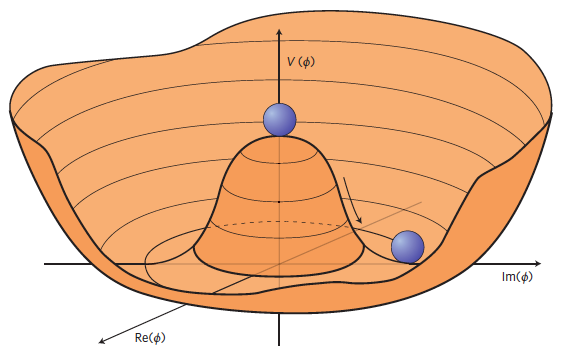
\includegraphics[width=0.8\linewidth]{higgspotential.png}
    \caption{Illustration of the Higgs potential \cite{Ellis:1638469}}
    \label{fig:Higgs_potential}
\end{figure}

The expansion of the ground state of the field $\Phi$ around the minimum can be parameterized with the real scalar field $h$ as:
\begin{equation}\label{eq:Higgs_field}
    \Phi(x) = \frac{1}{\sqrt{2}}\begin{pmatrix}
        0 \\
        v + h(x)
    \end{pmatrix}
\end{equation}
and finally, the potential $V(\Phi)$ can be rewritten as:
\begin{equation}
    V(\Phi) = - \lambda v^2 h^2(x) -\lambda vh^3(x) - \frac{\lambda}{4}h^4(x)
\end{equation}
The second and third terms represent the cubic and quartic self-coupling of the Higgs boson. Instead, from the first term, the value of the Higgs mass is obtained as:
\begin{equation}
    m_h^2 = \lambda v^2 = -2\mu^2
\end{equation}
In contrast to the weak boson self-interactions, which have a gauge nature, the Higgs boson self-interactions are purely related to the parameters of the scalar sector of the theory and entirely determined from the Higgs boson mass and the VEV. Consequently, their experimental measurement represents a crucial test of the validity and coherence of the SM.\\
\indent The massive gauge vector bosons can be obtained by replacing the vacuum expectation value of the $\Phi$ field in the EW Lagrangian with the additional invariant term due to the scalar field part. The H scalar field naturally acquires mass through self-interaction. When they interact with the vacuum, the gauge fields $W_\mu^1, W_\mu^2, W_\mu^3 $ gain a mass term in the form of $\frac{1}{2}M^2W_\mu W^\mu$, whereas the boson field associated with the photon remains massless. This means that despite breaking all the $SU(2) \otimes U(1)$ symmetries, the Higgs field maintains the $U(1)$ symmetry, leaving the vacuum electrically neutral. Remembering the relations in Equations (\ref{eq:Charged_boson}), (\ref{eq:Neutral_boson}) and (\ref{eq:Neutral_boson2}), the masses of the $W^\pm$ and Z bosons can be expressed with the weak coupling constants and the vacuum expectation value as:
\begin{equation}
    m_W = \frac{1}{2}vg \: \: \: \: \: \: \: \: \: \: \: \:  m_Z = \frac{1}{2}v\sqrt{g^2 + g'^2} = \frac{gv}{2\cos{\theta_W}} \: \: \: \: \: \: \: \: \: \: \: \: m_\gamma = 0
\end{equation}
The theory does not predict all the free parameters, nevertheless, the input is given from experimental values. For example, it is possible to determine the value of $v$, the scale of the electroweak theory, by measuring the Fermi constant $G_F$ from the muon lifetime \cite{Muon_lifetime}. $G_F$ is related to the W boson mass by $\frac{G_F}{\sqrt{2}} = \frac{g^2}{8m_W^2}$. The resulting value of $v$ is:
\begin{equation}
    v^2 = \frac{1}{\sqrt{2}G_F} \approx (246 \: GeV)^2
\end{equation}



\subsubsection{\label{subsec:intro_masses}Fermion masses}%
\noindent For weak interactions, the problem of massless particles does not only affect the bosons. Since under the $SU (2)_L$ left-handed particles transform as weak isospin doublets and right-handed particles as isospin singlets, the mass term of a spinor field written as chiral states also breaks the required gauge invariance. Even with the introduction of the spontaneous symmetry breaking mechanism and the Higgs field, fermion masses would still break gauge invariance under SU(2). Hence an additional mechanism has to be introduced in order to explain the massive fermions. As the Higgs field is responsible for the generation of boson masses, a mechanism is introduced that explains the origin of the fermion masses also via the interaction with the Higgs field. This interaction is called the Yukawa interaction \cite{Yukawa}, constituting a linear coupling of the Higgs field $\Phi$ with the fermion fields $\psi$,
\begin{equation}
    \mathscr{L}_{Yukawa, f} = - y_f \big( \overline{\psi}_L^f\Phi\psi_R^f + \overline{\psi}_R^f \Phi^{\dagger}\psi_L^f \big)
\end{equation}
where the superscript runs over all quarks and charged leptons. The different $y_f$ constants are known as Yukawa couplings of the particle $f$ to the Higgs field. For the electron $SU(2)$ doublet, the element with this coupling can be written as
\begin{equation}
    \mathscr{L}_e = -y_e\Bigg[(\overline{\nu}_e \: \overline{e})_L \begin{pmatrix}
        \phi_+ \\
        \phi_0
    \end{pmatrix} e_R + \overline{e}_R (\phi_+^* \: \phi_0^*) \begin{pmatrix}
        \nu_e \\ e
    \end{pmatrix}_L \Bigg]
\end{equation}
Here, obviously, $y_e$ denotes the Yukawa coupling of the electron to the Higgs boson. After spontaneously breaking the symmetry and thus using the expression of the Higgs field from Eq. (\ref{eq:Higgs_field}), the Lagrangian becomes:
\begin{equation} \label{eq:Yukawa_Lagrangian}
    \mathscr{L}_e = -\frac{vy_e}{\sqrt{2}}\overline{e}_Le_R -\frac{y_e}{\sqrt{2}}\overline{e}_Lhe_R -\frac{vy_e}{\sqrt{2}}\overline{e}_Re_L -\frac{y_e}{\sqrt{2}}\overline{e}_Rhe_L
\end{equation}
The first term of the Lagrangian in Eq. (\ref{eq:Yukawa_Lagrangian}) gives mass to the electron, which mass can be inferred as $m_e = y_ev/ \sqrt{2}$. The second term represents the coupling of the electron and the Higgs boson itself. No other interactions of fermions and the Higgs bosons or Higgs field are predicted by this formalism unlike for the bosons where also cubic and quartic interactions are predicted.\\
\indent The non-zero vacuum expectation value occurs only in the neutral part of the Higgs doublet due to the form in the ground state in Equation (\ref{eq:Higgs_field}). This implies that the combination $\overline{\psi}_L^f \Phi \psi_R^f + \overline{\psi}_R^f\Phi^\dagger\psi_L^f $ can only generate masses for the leptons in the lower component of an $SU(2)$ doublet. This explains why the neutrinos do not get mass through the Higgs mechanism.\\
\indent The process is analogous for quarks with the difference that, unlike the neutrinos, the up-type quarks do have right-chiral part. Thus, the Yukawa coupling of the fermions to the Higgs field is universally expressed as:
\begin{equation}
    y_f = \sqrt{2}\frac{m_f}{v}
\end{equation}
with $f$ being every fermion except the neutrinos, i.e., $ f ={e,\mu,\tau,d,u,s,c,b,t}$. It is obvious, that, from this mechanism, the mass of the fermions is determined by the Yukawa coupling constant $y_f$ and the VEV $v$. Therefore, in order to define the masses, which are not determined by the theory, the Yukawa couplings have to be measured experimentally. \\
\indent The measurement of the coupling of the fermions (and bosons) to the Higgs boson is an active field of study. While the coupling of the heaviest fermions to the Higgs boson has been established already, the couplings to lighter fermions still have to be measured. Due to the linear dependence of the Yukawa coupling strength to the mass of the fermion, the coupling measurements of lighter fermions are more difficult, as the small coupling strength is translated to lower rates of the process of interest. In Figure \ref{fig:Higgs_coupling}, the current state of coupling measurements of fermions and bosons to the Higgs boson is shown.\\
\begin{figure}[htb!]
    \centering
    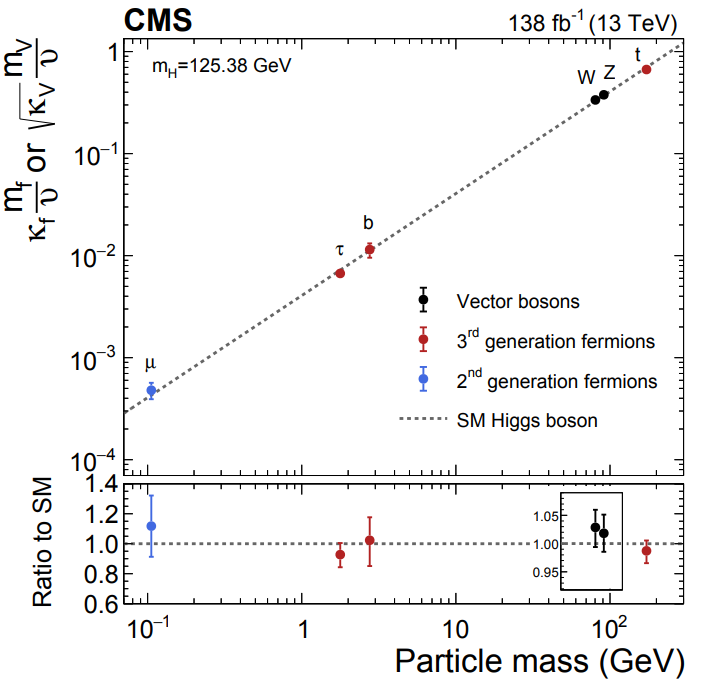
\includegraphics[width=0.75\linewidth]{Higgs_coupling.png}
    \caption{Coupling of fermions and bosons to the Higgs field \cite{Higgs_2022}}
    \label{fig:Higgs_coupling}
\end{figure}
\indent Finally, theoretical indications and experimental proofs have led to the conclusion that quarks as free particles are mass eigenstates but appear as SU(2) eigenstates in the electroweak interaction: the latter is a combination of the former, and vice versa \cite{Matsuoka_1998}. In particular, the introduction of quark mixing between EW q' and mass eigenstates q is needed to explain the experimental observation of the transitions between the upper and lower components of a quark flavor doublet across different families, e.g. from a u to a s quark, as well as the violation of charge and parity (CP) conservation in the SM \cite{10.1143/PTP.49.652, Cabibbo}. This implies that the quark flavor eigenstates do not coincide with the weak isospin eigenstates, but the lower components of the doublets are rotated relative to one another. More explicitly, the corresponding mixing between the lower components of the weak isospin eigenstates d', s' and b' are related to the lower components of the flavor eigenstates d, s and b as:

\begin{equation}
    \begin{pmatrix}
        d' \\ s' \\ b'
    \end{pmatrix} = \begin{pmatrix}
        V_{ud} & V_{us} & V_{ub} \\
        V_{cd} & V_{cs} & V_{cb} \\
        V_{td} & V_{ts} & V_{tb} 
    \end{pmatrix} \begin{pmatrix}
        d \\ s \\ b
    \end{pmatrix}
\end{equation}

The rotation matrix $V_{CKM}$ is the Cabibbo-Kobayashi-Maskawa (CKM) matrix describing the transition probabilities between flavors. In the SM, it is assumed to be unitary: the single matrix elements are free parameters of the theory, and all the values have been determined experimentally with very high precision \cite{alpigiani2017unitarity}. Large diagonal terms and small off-diagonal values characterize the CKM matrix. As a result, transitions between generations are significantly suppressed, and bottom quarks, for example, acquire a long lifetime. Additionally, as a consequence of quark mixing, flavor-changing neutral currents are not allowed at tree level \cite{PhysRevD.2.1285}, which explains why they are difficult to observe.\\
\indent The existence of the mixing is related to many physical examples, e.g. charge-parity (CP) violation, Glashow-Iliopoulos-Maiani (GIM) mechanism, flavor changing neutral currents (FCNC). However, an analogue of this matrix for the leptons is not present in the SM, since no right-handed neutrinos are included in the theory. Only because neutrino oscillations have been detected experimentally \cite{Fukuda_1998,Ahmad_2002,Agafonova_2018}, a similar mixing in the leptonic sector could be introduced to describe neutrinos as both flavor and mass eigenstates. This could be handled by the addition of a lepton mixing matrix, the Pontecorvo-Maki-Nakagawa-Sakata (PMNS) matrix \cite{10.1143/PTP.28.870, Pontecorvo:1957qd}, which emerges naturally as a consequence of the seesaw mechanism \cite{PhysRevLett.44.912} and has distinct phases depending on whether neutrinos are Dirac or Majorana particles \cite{BILENKY1980495}. The values of the masses of neutrinos are still unknown; however upper limits have been determined in experiments down to 0.8 eV \cite{aker2021direct}.

\section{\label{intro_top}The top quark}
\noindent The existence of the third-generation quarks was suggested to explain observations of CP violation. The observation of the b quark at Fermilab in 1977, confirmed the hypothesis and opened the quest for the top quark. The first experimental observation was reported independently by the CDF \cite{PhysRevLett.74.2626} and $D\cancel{0}$ \cite{PhysRevLett.74.2632} Collaborations in 1995 at the Fermilab Tevatron using proton-antiproton collisions at a center of mass energy of s = 1.8 TeV. \\
\indent The top quark (t) is the up-type quark of the third generation of fermions. Its most distinctive feature is its mass, which is the largest among all fundamental particles. The left-handed top quark is the Q = 2/3 and $I_3$ = +1/2 member of the weak isospin doublet that also contains the bottom quark. The right-handed top quark is the $SU(2)_L$ weak isospin singlet (Q = 2/3 and $I_3$ = 0). The top quark is often regarded as a window for new physics since it provides the highest natural energy scale to test the SM.
\subsubsection{Production mechanism}
\noindent The production of t$\overline{\text{t}}$ events via the strong interaction is the largest source of production of top quarks in hadron collisions as opposed to the single top production via the weak interaction. The t$\overline{\text{t}}$ process is one of the most important at LHC because it allows us to precisely study the properties of the top quark. Additionally, due to the dominance of this production mode, the t$\overline{\text{t}}$ production is also a major background in many measurements and searches for rare processes.\\
\indent At LHC, gluon fusion dominates with 90\% of the t$\overline{\text{t}}$ production. It is followed by the quark–antiquark annihilation, which accounts for 10\% of the total t$\overline{\text{t}}$ production. The leading-order Feynman diagrams are illustrated in Figure \ref{fig:tt}. When considering higher orders, the t$\overline{\text{t}}$ system is often accompanied by emissions of additional jets.\\
\begin{figure}[H]
    \centering
    %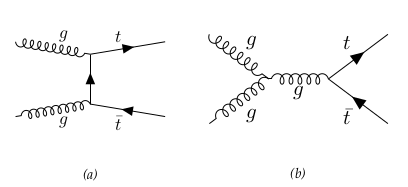
\includegraphics[width=0.6\linewidth]{tt.png}
    \begin{subfigure}[b]{0.45\textwidth}
    \centering
    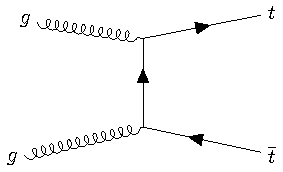
\includegraphics[width=0.75\linewidth]{tt.pdf}
    \caption{}
  \end{subfigure}
  %
  \begin{subfigure}[b]{0.45\textwidth}
    \centering
    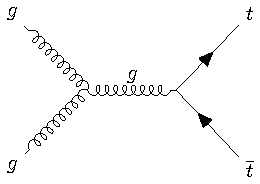
\includegraphics[width=0.75\linewidth]{tt_2.pdf}
    \caption{}
  \end{subfigure}
    \caption{Feynman diagrams for top quark pair production processes at leading order}
    \label{fig:tt}
\end{figure}
\indent The t$\overline{\text{t}}$ production cross section has been studied at various center-of-mass energies for p-p collisions. The measurements are compared to the theoretical prediction, showing good agreement as in Figure \ref{fig:tt_cross_section}. For $\sqrt{s} $= 13 TeV, the predicted t$\overline{\text{t}}$ cross section for $m_t = 172.5$ GeV is \cite{LHCTopWG}: 
\begin{equation}
    \sigma_{t\overline{t}} = 833.9^{+20.5}_{-30.0}\text{(scale)}\pm 21.0\text{(PDF + $\alpha_s$)}^{+23.18}_{-22.45} \text{(mass) pb}
\end{equation}
\begin{figure}[H]
    \centering
    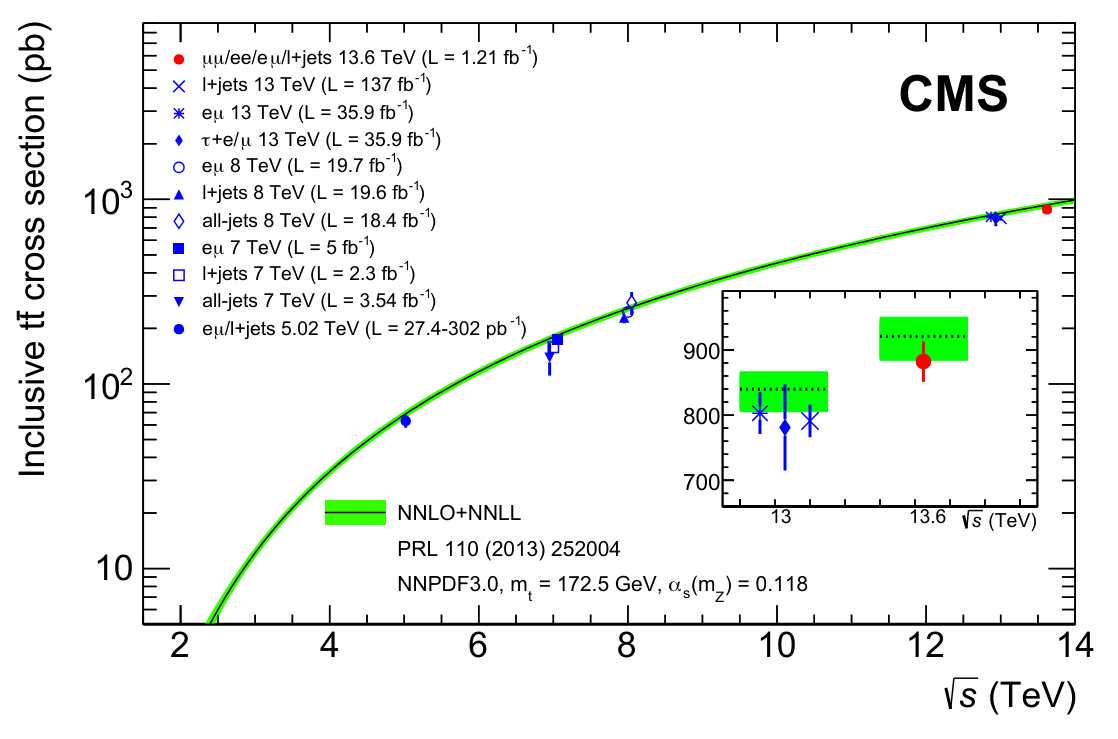
\includegraphics[width=0.8\linewidth]{tt_cross_section.png}
    \caption{Cross section of t$\overline{\text{t}}$ production as a function of the center-of-mass energy at the CMS experiment \cite{2023_tt_X}}
    \label{fig:tt_cross_section}
\end{figure}
\subsubsection{Decay mechanism}
\noindent Due to its large mass, the top quark decays with a lifetime of $\tau_t = 5\times 10^{-25}$ s \cite{Workman:2022ynf}. Actually, it is shorter than its hadronization timescale (1/$\Lambda_{QCD} \sim 10^{-24}$ s). This represents an opportunity to study quarks in a free state, something that is quite exceptional due to color confinement, as explained in Section \ref{intro_QCD}. In fact, the top quark is the only quark that can be investigated unbounded. Its lifetime is also smaller than the spin decorrelation timescale ($m_t/\Lambda^2_{QCD} \sim 10^{-21}$ s \cite{PhysRevD.81.074024}, $m_t$ being the mass of the top quark), implying that the top-quark states conserve their spin state from its production to its decay. Therefore, the top-quark properties, such as the spin information and the top-quark polarization, can also be accessed through its decay products and, consequently, be measured.\\
\indent Due to the large value of the $V_{tb}$ element of the CKM matrix, the top quark is expected to decay almost entirely ($\sim 99.8\% $) to a b quark and a W boson ($t \rightarrow Wb$). The final-state decay is classified according to the subsequent decay of the W boson. Since the W bosons are massive vector bosons, their lifetime is very short ($\tau_W \approx 3 \times 10^{-25}$ s) and hence they will rapidly decay to leptons or quarks that will form hadrons. Due to its large mass, the W boson can decay to any quark except the top quark. For the $W^+$, the branching ratios\footnote{For each decay mode, the branching ratio (BR) is defined as the fraction times that the particle decays in that particular mode with respect to total possible decays.} (BRs) for the different decay modes are presented in Table \ref{tab:W_decays}
\begin{table}[H]
\centering
\caption{W-boson-decay branching ratios \cite{Workman:2022ynf}}
\label{tab:W_decays}
\begin{tabular}{lc}
\hline
Decay mode                                & Branching ratio [\%] \\ \hline
$W^+ \rightarrow e^+\nu_e$                & $10.71 \pm 0.16$    \\
$W^+ \rightarrow \mu^+ \nu_\mu$           & $10.63 \pm 0.15$    \\
$W^+ \rightarrow \tau^+ \nu_\tau$         & $11.38 \pm 0.21$    \\
$W^+ \rightarrow q\overline{q}$ (hadrons) & $67.41 \pm 0.27$    \\
$W^+ \rightarrow $ invisible              & $1.4 \pm 2.9$      
\end{tabular}
\end{table}
For the conjugate process involving the $W^-$, the BRs are the same. Therefore, the W boson decay and consequently the top-quark decay can be classified either as leptonic or hadronic.
\subsubsection{Decay channels}
\noindent There are three different decay channels of the t$\overline{\text{t}}$, depending on the decay of the W-bosons:
\begin{itemize}
    \item \textbf{Fully-Hadronic (FH)}: Both W bosons decay into quarks, mostly as $W^+/W^- \rightarrow u\overline{d}/\overline{u}d$ and $W^+/W^- \rightarrow c\overline{s}/\overline{c}s$, they hadronize and lead to the experimental signature of six jets in the final state. Although this decay mode has a relatively high branching ratio of approximately 46\% at parton level and $\approx$55\% at hadron level, its analysis is challenging due to significant background contributions from multijet processes and the combinatorial ambiguities in the reconstruction of the events. 
    \item \textbf{Semi-Leptonic (SL)}: Only one W decays into hadrons and the other decays into leptons: the final state comprises four jets, one charged lepton and one neutrino in the final state. The branching ratio is approximately 45\% at parton level and $\approx$38\% at hadron level, but the multijet background is significantly suppressed by the isolation requirements on the charged lepton. Furthermore, to reconstruct the complete event kinematics, the momentum vector of a single neutrino can be retrieved with good efficiency from a missing transverse momentum measurement in combination with a constraint on the W boson mass.
    \item \textbf{Di-Leptonic (DL)}: Both W bosons decay into leptons: the final state features two jets, two oppositely-charged leptons and two neutrinos. The combined branching ratio $\approx$9\% at parton level and $\approx$7\% at hadron level, is the smallest, but the signature is distinct. The full event reconstruction is challenging because the neutrinos are neither detectable nor unambiguously retrievable utilizing the missing transverse momentum balance. 
\end{itemize}
% \subsection{\label{top:pair-production}Top-quark-antiquark pairs production}
% The gluon-gluon fusion processes account for approximately 90\% of the t$\overline{\text{t}}$ cross section for p-p collisions [55]. The leading-order Feynman diagrams are illustrated in Figure 1.14 (a)
% and (b). When considering higher orders, the tt system is often accompanied by emissions of
% additional jets.


\section{\label{intro_Higgs}The Higgs boson}
\noindent The Higgs boson represents the quantum of the scalar field introduced in Section \ref{sec:intro_symmetry}, in the discussion of the electroweak symmetry breaking. In the SM, the Higgs boson is expected to be electrically neutral, free of spin, and CP-even ($\mathit{JP} = 0^+$) with a decay width of approximately 4 MeV. \\
\indent The signatures for SM Higgs boson detection at collider experiments depend on the production process and the decay pattern. Both the production and the decay contribute to the specific kinematic features which can be used to distinguish signal from the background events.\\
\indent A multitude of experimental searches on Higgs boson were performed during the first run period of LHC with proton-proton collisions at $\sqrt{s} = 7, 8$ TeV. On 4 July 2012, the observation of a new particle at a mass of approximately 125 GeV with Higgs boson-like properties was finally reported by the CMS \cite{Higgs1} and ATLAS \cite{Higgs2} Collaborations with integrated luminosity of 5.1 (5.3) $\text{fb}^{-1}$ at 7 (8) TeV. Subsequent measurements of the new particle properties such as spin, parity, and coupling strength to SM particles are found to be consistent, within the experimental uncertainties, with the expectation for the SM Higgs boson \cite{Aad2016, Khachatryan2015, 2013120, PhysRevD.92.012004}. The full Run-II dataset collected during the LHC proton-proton collisions at a higher energy $\sqrt{s}$ = 13 TeV provides more statistical power to further constrain the Higgs boson mass measurement and elucidate other production and decay modes.
\subsubsection{\label{subsubsec:Production_mechanisms}Production mechanisms}
\noindent One of the reasons the Higgs boson was the last of the SM’s fundamental particles to be discovered is its relatively high mass, which required significant energy for its production. Even in high-energy collisions, the production of a Higgs boson is a rare event. Only a tiny fraction of collisions at the LHC produce a Higgs boson, so vast numbers of collisions had to be analysed to find the Higgs boson.\\
\begin{figure}[H]
  \centering
  \begin{subfigure}[b]{0.45\textwidth}
    \centering
    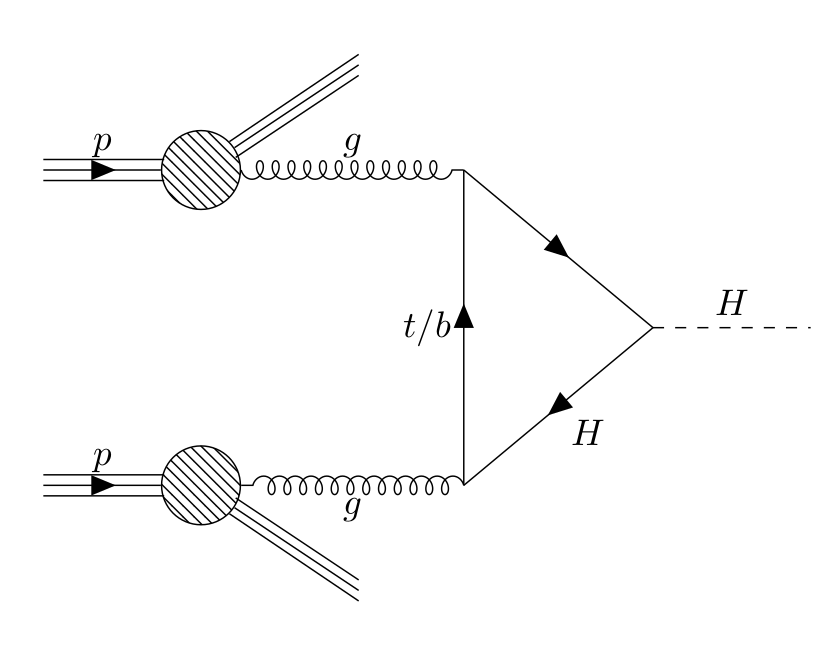
\includegraphics[width=1.0\linewidth]{ggF.png}
    % \begin{tikzpicture}
    %   \begin{feynman}
    %     \vertex (a) {\(\mu^{-}\)};
    %     \vertex [right=of a] (b);
    %     \vertex [above right=of b] (f1) {\(\nu_{\mu}\)};
    %     \vertex [below right=of b] (c);
    %     \vertex [above right=of c] (f2) {\(\overline \nu_{e}\)};
    %     \vertex [below right=of c] (f3) {\(e^{-}\)};
    
    %     \diagram* {
    %       (a) -- [fermion] (b) -- [fermion] (f1),
    %       (b) -- [boson, edge label'=\(W^{-}\)] (c),
    %       (c) -- [anti fermion] (f2),
    %       (c) -- [fermion] (f3),
    %     };
    %   \end{feynman}
    % \end{tikzpicture}
    \caption{}
  \end{subfigure}
  %
  \begin{subfigure}[b]{0.45\textwidth}
    \centering
    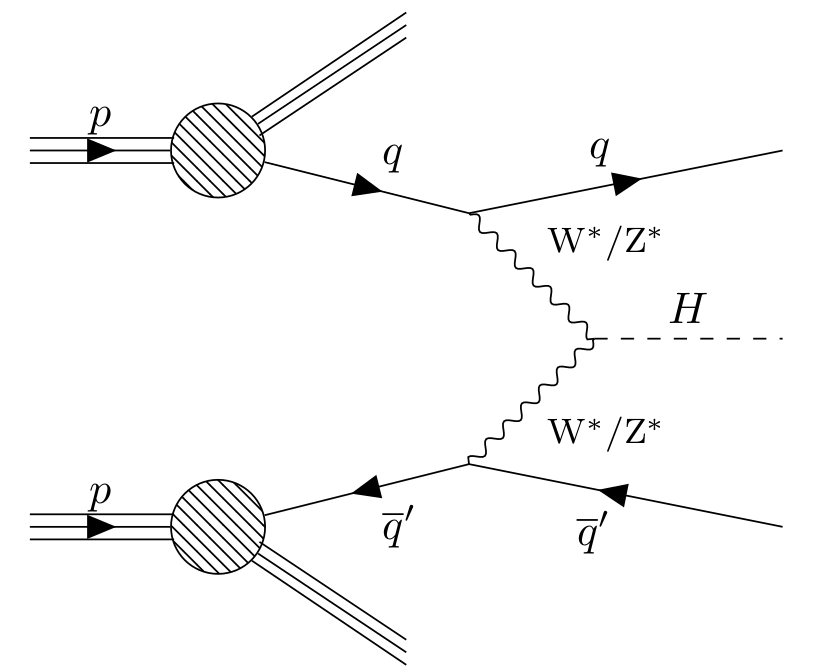
\includegraphics[width=1.0\linewidth]{VBFusion.png}
    % \begin{tikzpicture}
    %   \begin{feynman}
    %     \vertex (a) {\(\mu^{-}\)};
    %     \vertex [right=of a] (b);
    %     \vertex [above right=of b] (f1) {\(\nu_{\mu}\)};
    %     \vertex [below right=of b] (c);
    %     \vertex [above right=of c] (f2) {\(\overline \nu_{e}\)};
    %     \vertex [below right=of c] (f3) {\(e^{-}\)};
    
    %     \diagram* {
    %       (a) -- [fermion] (b) -- [fermion] (f1),
    %       (b) -- [boson, edge label'=\(W^{-}\)] (c),
    %       (c) -- [anti fermion] (f2),
    %       (c) -- [fermion] (f3),
    %     };
    %   \end{feynman}
    % \end{tikzpicture}
    \caption{}
  \end{subfigure}
  
  \vspace{1cm}
  
  \begin{subfigure}[b]{0.45\textwidth}
    \centering
    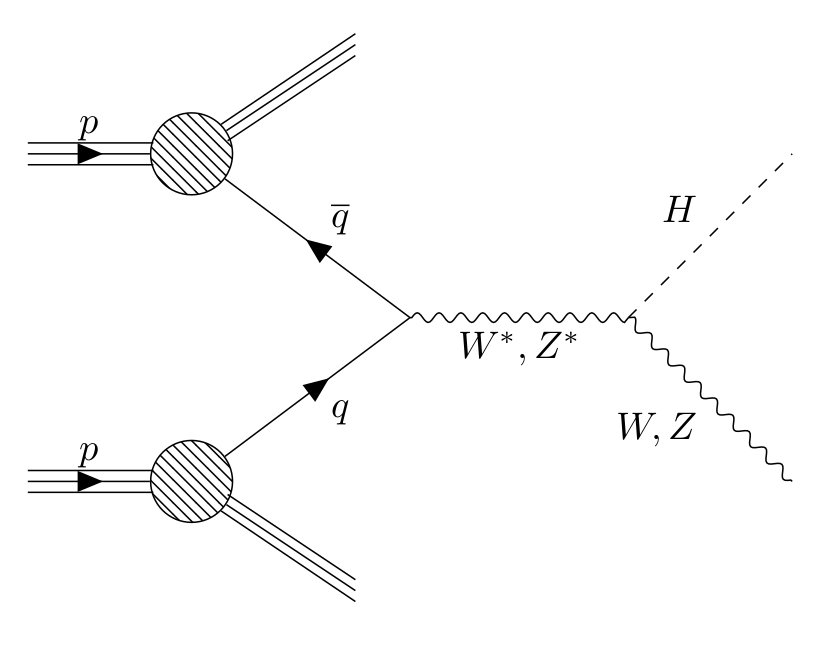
\includegraphics[width=1.0\linewidth]{Higgsstrahlung.png}
    % \begin{tikzpicture}
    %   \begin{feynman}
    %     \vertex (a) {\(\mu^{-}\)};
    %     \vertex [right=of a] (b);
    %     \vertex [above right=of b] (f1) {\(\nu_{\mu}\)};
    %     \vertex [below right=of b] (c);
    %     \vertex [above right=of c] (f2) {\(\overline \nu_{e}\)};
    %     \vertex [below right=of c] (f3) {\(e^{-}\)};
    
    %     \diagram* {
    %       (a) -- [fermion] (b) -- [fermion] (f1),
    %       (b) -- [boson, edge label'=\(W^{-}\)] (c),
    %       (c) -- [anti fermion] (f2),
    %       (c) -- [fermion] (f3),
    %     };
    %   \end{feynman}
    % \end{tikzpicture}
    \caption{}
  \end{subfigure}
  %
  \begin{subfigure}[b]{0.45\textwidth}
    \centering
    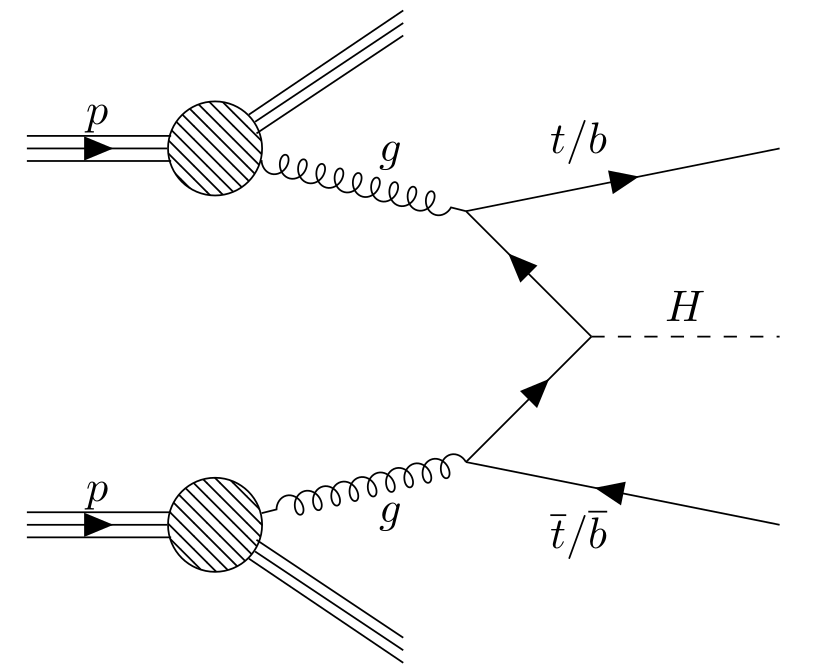
\includegraphics[width=1.0\linewidth]{ttH.png}
    % \begin{tikzpicture}
    %   \begin{feynman}
    %     \vertex (a) {\(\mu^{-}\)};
    %     \vertex [right=of a] (b);
    %     \vertex [above right=of b] (f1) {\(\nu_{\mu}\)};
    %     \vertex [below right=of b] (c);
    %     \vertex [above right=of c] (f2) {\(\overline \nu_{e}\)};
    %     \vertex [below right=of c] (f3) {\(e^{-}\)};
    
    %     \diagram* {
    %       (a) -- [fermion] (b) -- [fermion] (f1),
    %       (b) -- [boson, edge label'=\(W^{-}\)] (c),
    %       (c) -- [anti fermion] (f2),
    %       (c) -- [fermion] (f3),
    %     };
    %   \end{feynman}
    % \end{tikzpicture}
    \caption{}
  \end{subfigure}

  \caption{Feynman diagrams at leading order for Higgs boson production via (a) gluon-gluon fusion, (b) vector boson fusion (c) Higgsstrahlung and (d) associate production with heavy quarks.}
  \label{fig:Higgs_production_feynman diagrams}
\end{figure}
\indent The four dominant processes for Higgs-boson production at LHC are summarised in Figure \ref{fig:Higgs_production_feynman diagrams}. These processes are:

% \large
% \begin{fmffile}{feyngraph}
%   \begin{fmfgraph*}(150,60)
%     \fmfstraight
%     \fmfleft{i1,i2}
%     \fmfright{o1,h,o2}
%     % gluons
%     \fmf{gluon}{i1,t1}
%     \fmf{gluon}{t2,i2}
%     \fmf{phantom,tension=0.5}{t1,o1}
%     \fmf{phantom,tension=0.5}{t2,o2}
%     \fmffreeze
%     % top loop
%     \fmf{fermion,tension=1}{t1,t2,t3,t1}
%     % Higgs boson
%     \fmf{dashes,tension=2.0}{t3,h}
%     % labels
%     \fmflabel{$g$}{i1}
%     \fmflabel{$g$}{i2}
%     \fmflabel{H}{h}
%   \end{fmfgraph*}
% \end{fmffile}


\begin{itemize}
    \item \textbf{Gluon-gluon fusion} (ggF): The process $gg \rightarrow H$ has to be mediated by a massive fermion loop. This is due to the fact that there is no direct gluon-Higgs-boson coupling within the SM. Although in principle all quarks should be included in the loop, in practice it is the top quark the one doing so because its coupling to the Higgs boson is 40 times stronger than the next-heaviest fermion, the bottom quark. Due to the abundance of gluons in pp collisions, the ggF is very favoured at the LHC.
    \item \textbf{Vector boson fusion} (VBF): The second most important mode is the radiation by the incoming quarks of a pair of W or Z bosons that fuse to form a Higgs boson. The vector bosons (V = W or Z ) of the process $V\overline{V} \rightarrow H$ are originated from initial state quarks which scatter through the final state (changing their flavors in the case of W fusion) producing two forward jets.
    \item \textbf{Higgsstrahlung} (VH): There is another significant contribution involving the W or Z bosons, the Higgsstrahlung or associated $W H$ or $Z H$ production. Here, an off-shell W or Z boson (formed from the annihilation of two quarks) radiates a Higgs boson via $V^* \rightarrow VH$.
    \item  \textbf{Quark-pair associated production} (q$\overline{\text{q}}$H): In this mode, the Higgs is produced from a q$\overline{\text{q}}$ pair via $q\overline{q} \rightarrow H$ with a q$\overline{\text{q}}$ final state. Typically, the involved quark pair is either a b$\overline{\text{b}}$ or t$\overline{\text{t}}$. In the case of t$\overline{\text{t}}$ , the top quarks decay before hadronizing, leading to final states with a high number of physics objects.
\end{itemize}

\indent The cross-section of the different mechanisms for single-Higgs-boson production at $\sqrt{s} = 13$ TeV as a function of $m_H$ are shown in Figure \ref{fig:Higgs_cross_section}, while assuming a $m_H = 125.2$ GeV, the Higgs-boson production cross-sections for the different modes are presented in Table \ref{tab:Higgs_production}.
\begin{table}[H]
\small
\caption{Higgs-boson-production cross sections assuming $m_H$ = 125.2 GeV for a LHC CM energy of $\sqrt{s}$ = 13 TeV \cite{Higgs_production}.} 
\centering
\label{tab:Higgs_production}
\begin{tabular}{cc}
\hline
Production mode  & Cross section [pb]     \\ \hline
ggF              & $48.44^{+2.72}_{-3.60}$  \\ %N3LO QCD
VBF              & $3.78\pm 0.08$   \\ %NNLO
WH               & $1.37\pm 0.03$   \\ %NLO QCD +EW
ZH               & $0.89 \pm 0.04$ \\ %NLO QCD +EW 
t$\overline{\text{t}}$H & $0.51 \pm 0.04$  \\
$b\overline{b}H$ & $0.49 \pm 0.1$    %NNLO(5FS) NLO(4FS)
\end{tabular}
\end{table}
\begin{figure}[H]
    \centering
    \begin{subfigure}{0.49\textwidth}
        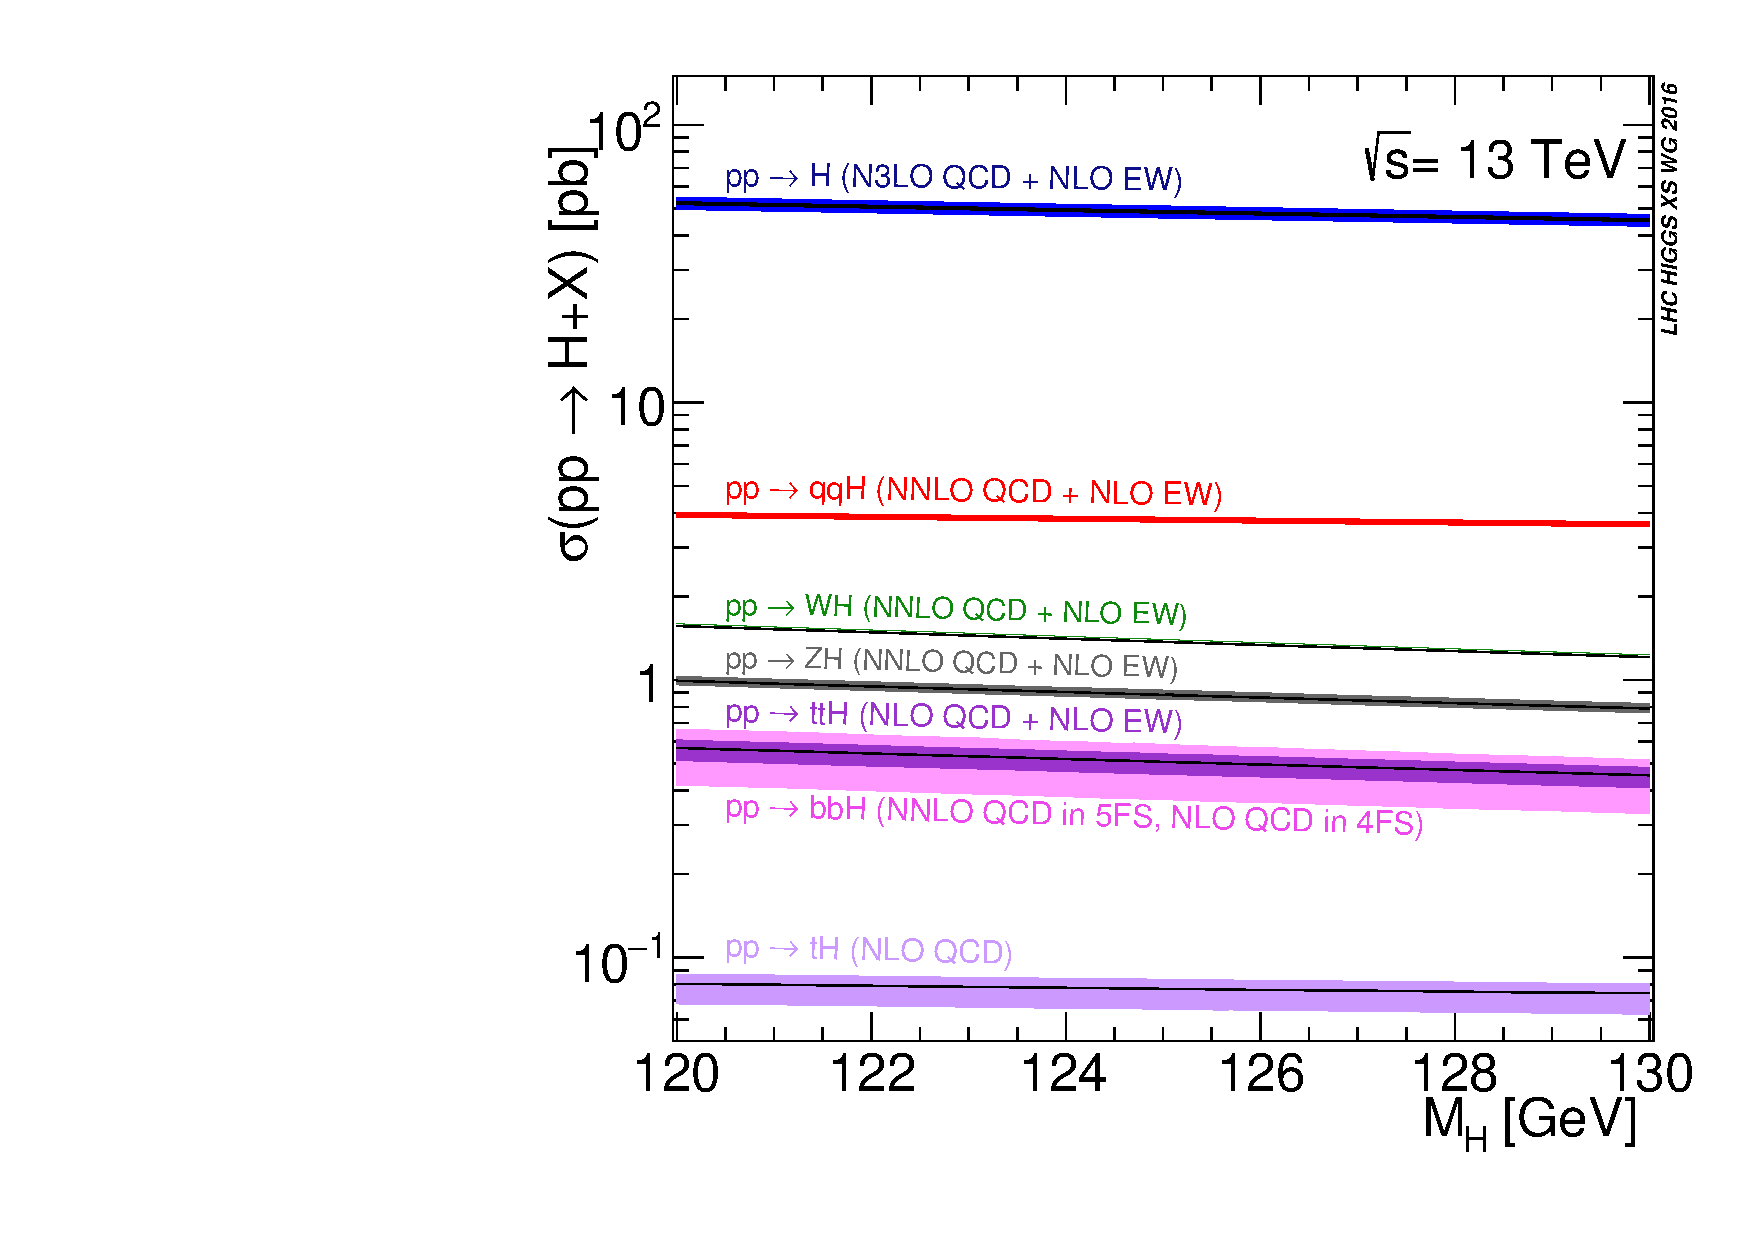
\includegraphics[width=1.0\linewidth]{plot_13tev_H_sqrt.pdf}
        \caption{}
        \label{fig:Higgs_cross_section}
    \end{subfigure}
    \begin{subfigure}{0.49\textwidth}
        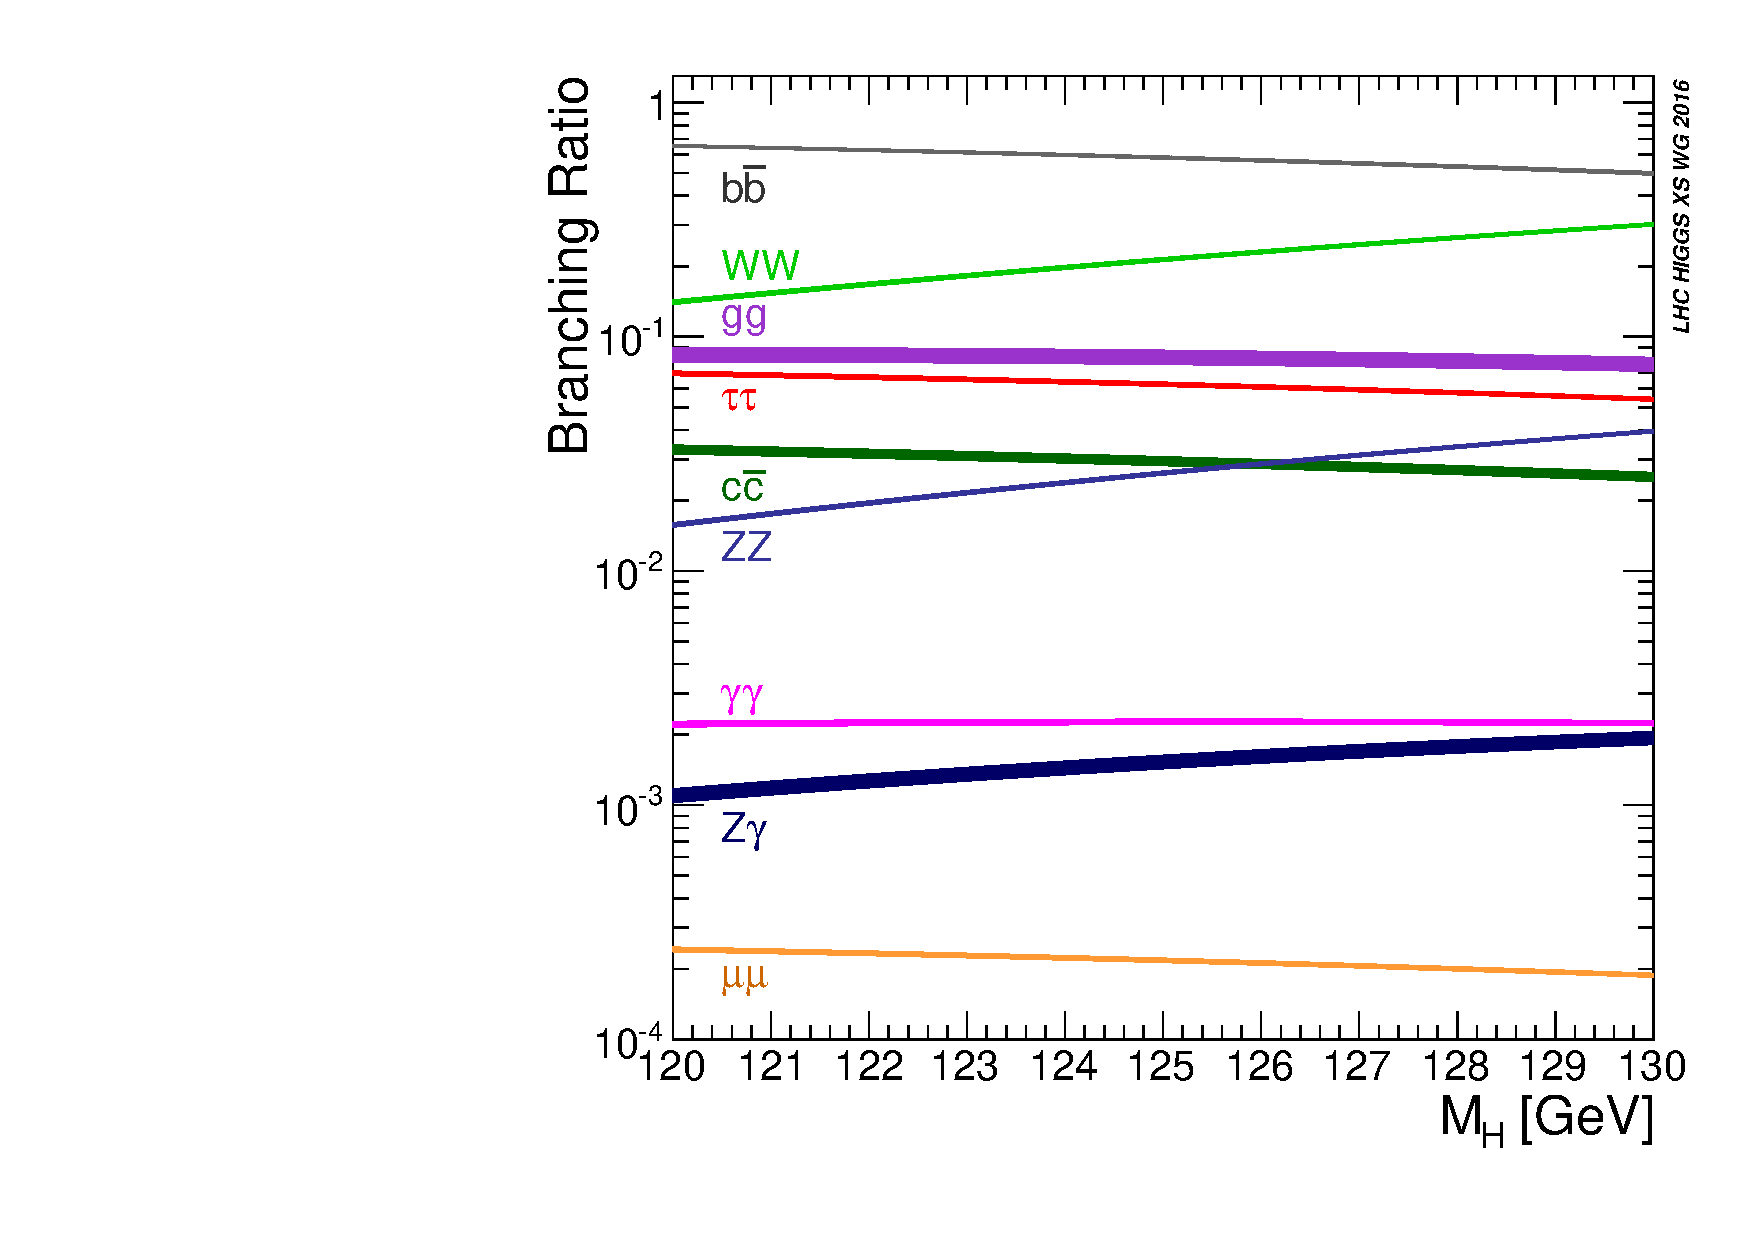
\includegraphics[width=1.0\linewidth]{SMHiggsBR.YR4-square.pdf}
        \caption{}
        \label{fig:Higgs_BR}
    \end{subfigure}
    \caption{Higgs-boson (a) production cross sections and (b) branching ratios as a function of $m_H$ at $\sqrt{s}$ = 13 TeV \cite{Higgs_production}}
    \label{fig:Higgs_XS_BR}
\end{figure}



\subsubsection{\label{subsubsec:Higgs_Decay_channels}Decay channels}
\noindent The Higgs boson has a very short lifetime ($\tau_H = 1.6 \times 10^{-22}$ \cite{Higgs_production}) and hence, is always detected through its decay products. Figure \ref{fig:Higgs_BR} shows the branching ratio as a function of $m_H$ for the different Higgs-boson decay modes.\\
% \begin{figure}[H]
%     \centering
%     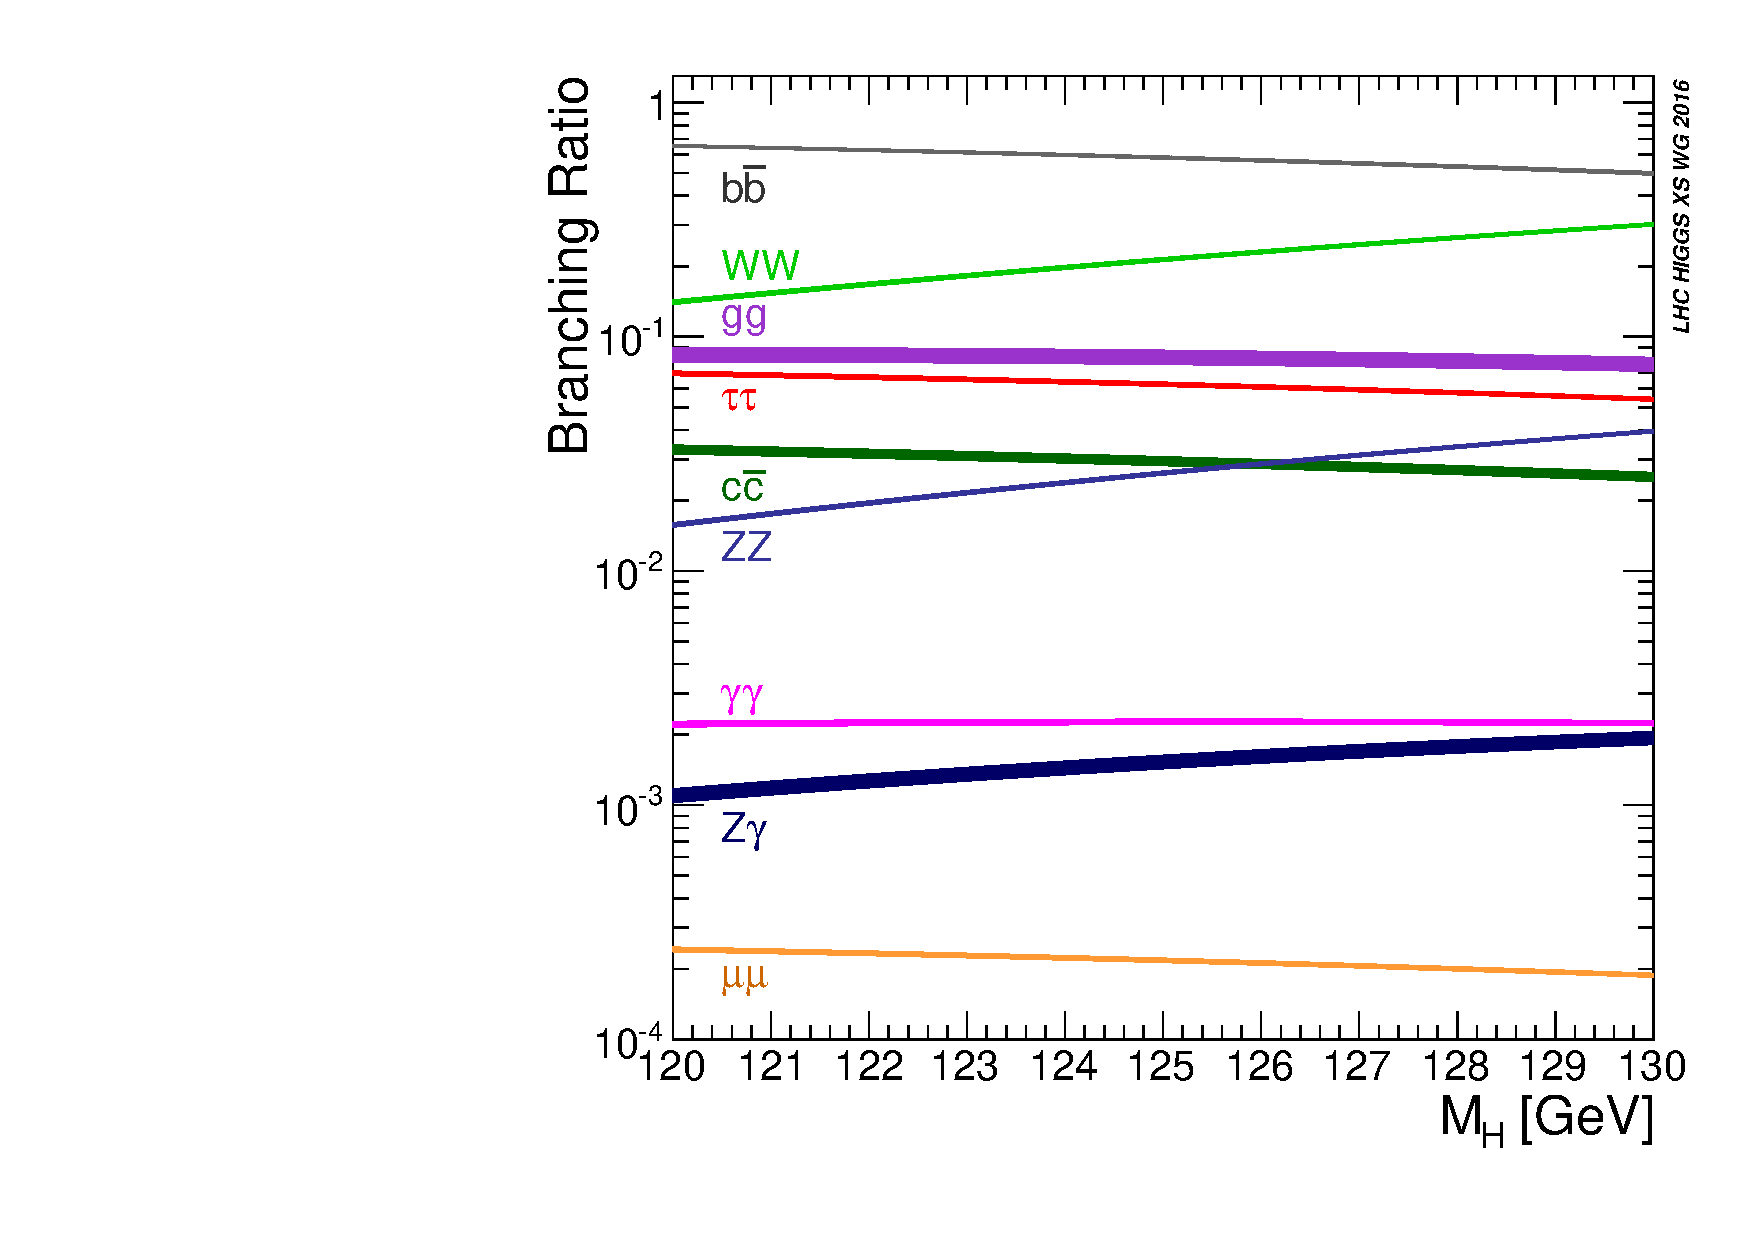
\includegraphics[width=0.5\linewidth]{SMHiggsBR.YR4-square.pdf}
%     \caption{Higgs-boson-decay branching ratios as a function of $m_H$ at $\sqrt{s}$ = 13 TeV \cite{Higgs_production}}
%     \label{fig:Higgs_BR}
% \end{figure}
\begin{table}[H]
\centering
\small
\caption{Higgs-boson-decay branching ratios assuming $m_H$ = 125.2 GeV at NLO \cite{Higgs_production}}
\label{tab:Higgs_decays}
\begin{tabular}{lc}
\hline
Decay mode                    & Branching ratio [\%] \\ \hline
$H \rightarrow b\overline{b}$ & $57.92 \pm 0.007$  \\
$H \rightarrow W^+ W^-$        & $21.70 \pm 0.003$       \\
$H \rightarrow gg$            & $8.172 \pm 0.004$        \\
$H \rightarrow\tau^-\tau^+$   & $6.240 \pm 0.001$        \\
$H \rightarrow c\overline{c}$ & $2.876 \pm 0.002$      \\
$H \rightarrow ZZ$            & $2.667 \pm 0.001$      \\
$H \rightarrow \gamma\gamma$  & $0.227 \pm 0.001$      \\
$H \rightarrow Z\gamma$       & $0.155 \pm 0.003$      \\
$H \rightarrow \mu^-\mu^+$    & $0.02165 \pm 0.00004$                
\end{tabular}
\end{table}
\indent Despite the expected large Yukawa coupling between the Higgs boson and the top quark, the $H \rightarrow t\overline{t} $ is forbidden since $m_H < 2m_t$ . Consequently, the most prominent decay mode is $H \rightarrow b\overline{b}$ followed by $H \rightarrow W^+ W^-$. This is why for the $tHq$ searches, the channel in which the Higgs decay to b$\overline{\text{b}}$ is the one with higher statistics. For the other fermionic decays, the decay rates are ordered by the fermion masses, with $\tau^+\tau^-$ decay mode being the biggest among the leptonic ones. Regardless of the expected large coupling between the weak-force bosons and the Higgs boson, the $H \rightarrow VV^*$ is suppressed due to the requirement that one vector boson has to be produced off-shell\footnote{Off-shell means that the particle is produced virtually and it does not satisfy the energy-momentum relation: $E^2 = p^2 + m^2$.}.\\
\indent Sorted by importance and assuming a Higgs-boson mass equal to 125.2 GeV, the BRs for the Higgs boson are listed in Table \ref{tab:Higgs_decays}.
% \begin{figure}[H]
%   \centering
%   \begin{subfigure}{0.45\textwidth}
%     \centering
%     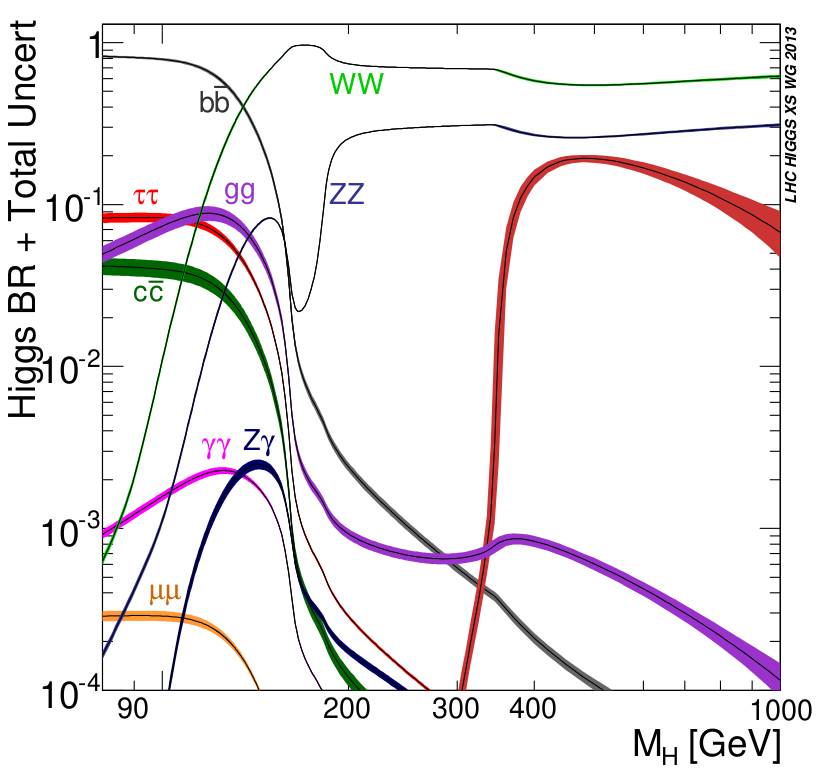
\includegraphics[width=1.0\linewidth]{Higgs_BR.png}
%      \caption{}
%     \label{fig:Higgs_BR1}
%   \end{subfigure}
%   \hfill
%   \begin{subfigure}{0.47\textwidth}
%     \centering
%     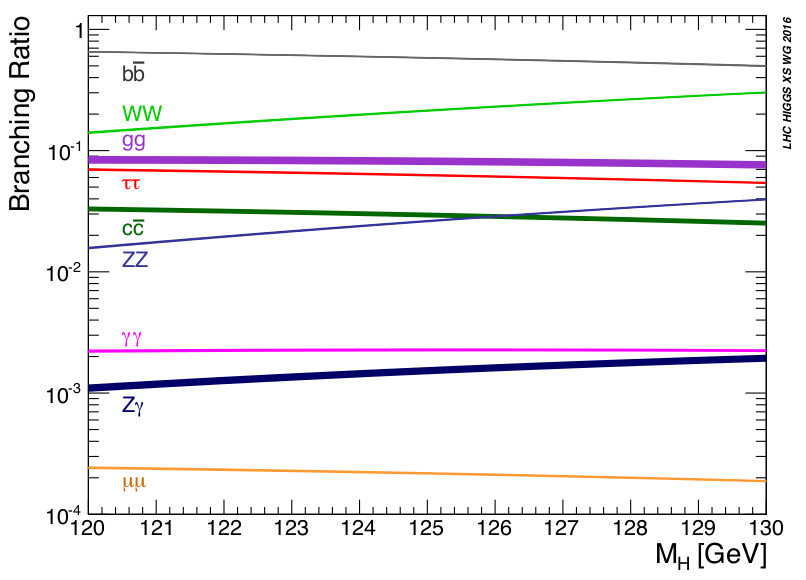
\includegraphics[width=1.0\linewidth]{Higgs_BR2.png}
%      \caption{}
%     \label{fig:Higgs_BR2}
%   \end{subfigure}
%   \caption{(a) (b)}
%   \label{fig:Higgs_BR}
% \end{figure}





\section{\label{intro_ttH}Associated top-pair and Higgs-boson production}
\begin{figure}[H]
    \centering
    \begin{subfigure}{0.45\textwidth}
        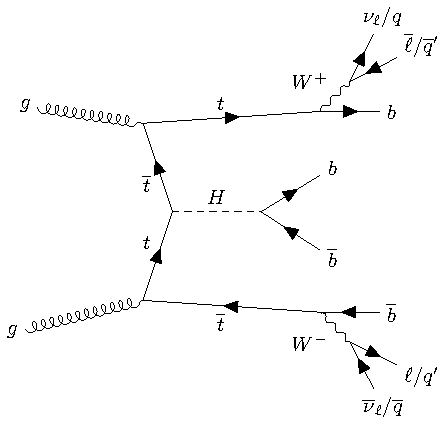
\includegraphics[width=1.0\linewidth]{ttHbb_fs.pdf}
        \caption{}
    \end{subfigure}
    \begin{subfigure}{0.45\textwidth}
        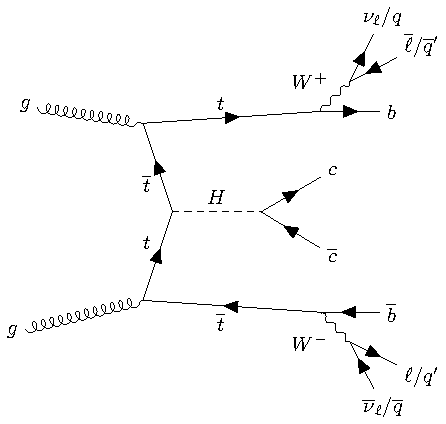
\includegraphics[width=1.0\linewidth]{ttHcc_fs.pdf}
        \caption{}
    \end{subfigure}
    \caption{Feynman diagrams of the t$\overline{\text{t}}$H process with all possible final states of the t$\overline{\text{t}}$ system  with the Higgs boson decaying to (a) a pair of b quarks and (b) a pair of c quarks.}
    \label{fig:ttH}
\end{figure}
\noindent The associated production of a Higgs boson and a top quark-antiquark pair (t$\overline{\text{t}}$H) provides a direct probe of the top-Higgs coupling as illustrated by the Feynman diagram in Fig. \ref{fig:ttH}, and has recently been observed by the ATLAS and CMS Collaborations \cite{ttH_1,ttH_2}. Moreover, Higgs boson decays to pairs of bottom quarks have also been observed \cite{ttH_3,ttH_4}, thereby directly probing the Yukawa interactions between the Higgs boson and top as well as bottom quarks for the first time. Overall, the observed interactions with gauge bosons and third-generation fermions, alongside all measured properties, are consistent with the predictions of the Standard Model. One of the upcoming key objectives of the LHC physics program is to investigate interactions involving second generation fermions. The CMS Collaboration recently announced initial findings of Higgs boson decays into muons \cite{Sirunyan_2021}. A critical upcoming milestone is observing its coupling to second-generation quarks and more specifically the coupling to the charm quark. In order to achieve this, ATLAS and CMS Collaborations target the associated production of a Higgs boson with a top quark-antiquark pair, where the Higgs boson decay to a charm quark-antiquark pair. However, the small branching fraction predicted by the SM, ubiquitous production of quark and gluon jets at the LHC, and the difficulty of identifying charm quark jets in a hadronic environment, including distinguishing them from bottom quark jets, make this a challenging measurement.

% \subsubsection{Decay channels}
% \noindent There are three different decay channels of the t$\overline{\text{t}}$H intermediate state, depending on the decay of the W-bosons:
% \begin{itemize}
%     \item \textbf{Fully-Hadronic (FH)}: Both W bosons decay into quarks, mostly as $W^+/W^- \rightarrow u\overline{d}/\overline{u}d$ and $W^+/W^- \rightarrow c\overline{s}/\overline{c}s$, they hadronize and lead to the experimental signature of six jets in the final state. Although this decay mode has a relatively high branching ratio of approximately 46\% at parton level and $\approx$55\% at hardon level, its analysis is challenging due to significant background contributions from multijet processes and the combinatorial ambiguities in the reconstruction of the events. 
%     \item \textbf{Semi-Leptonic (SL)}: Only one W decays into hadrons and the other decays into leptons: the final state comprises four jets, one charged lepton and one neutrino in the final state. The branching ratio is approximately 45\% at parton level and $\approx$38\% at hardon level, but the multijet background is significantly suppressed by the isolation requirements on the charged lepton. Furthermore, to reconstruct the complete event kinematics, the momentum vector of a single neutrino can be retrieved with good efficiency from a missing transverse momentum measurement in combination with a constraint on the W boson mass.
%     \item \textbf{Di-Leptonic (DL)}: Both W bosons decay into leptons: the final state features two jets, two oppositely-charged leptons and two neutrinos. The combined branching ratio $\approx$9\% at parton level and $\approx$7\% at hardon level, is the smallest, but the signature is distinct. The full event reconstruction is challenging because the neutrinos are neither detectable nor unambiguously retrievable utilizing the missing transverse momentum balance. 
% \end{itemize}

\subsection{\label{intro_ttbb}Associated top-pair and heavy-flavored jets production}
\noindent The dominant background for t$\overline{\text{t}}$H process arises from pure top quark production. In the case of additionally emitted jets (t$\overline{\text{t}}$ + jets), mostly heavy-flavor jets (t$\overline{\text{t}}$ + b$\overline{\text{b}}/$c$\overline{\text{c}}$), the process has very similar final-state content and kinematic topology as the t$\overline{\text{t}}$H, H $\rightarrow$ b$\overline{\text{b}}/$c$\overline{\text{c}}$ one.\\
\indent In fact, analogously to the t$\overline{\text{t}}$H, we can define the same three decay channels since we have again t$\overline{\text{t}}$ as an intermediate state, while the additionally emitted jets correspond to the jets produced from the Higgs decay, resulting in the exact same (but non-resonant) final states, as shown in Fig. \ref{fig:ttbb}.
\begin{figure}[H]
    \centering
    \begin{subfigure}{0.45\textwidth}
        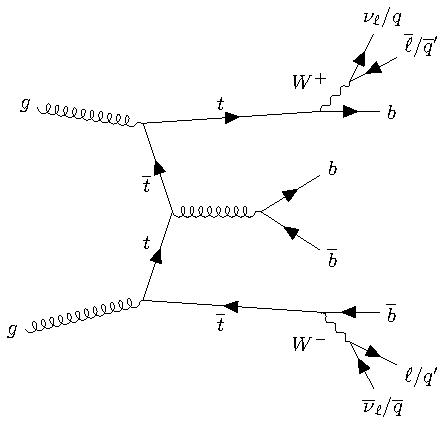
\includegraphics[width=1.0\linewidth]{ttbb_fs.pdf}
        \caption{}
    \end{subfigure}
    \begin{subfigure}{0.45\textwidth}
        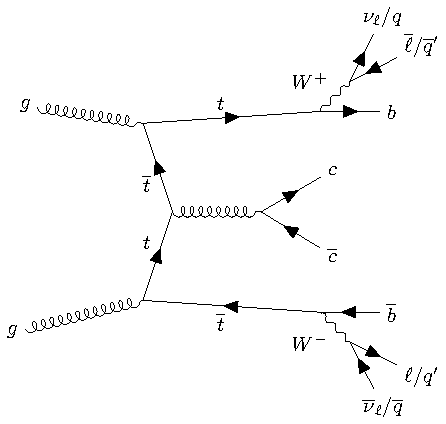
\includegraphics[width=1.0\linewidth]{ttcc_fs.pdf}
        \caption{}
    \end{subfigure}
    \caption{Feynman diagrams of the t$\overline{\text{t}}$ + jets process with all possible final states of the t$\overline{\text{t}}$ system  with the addition of emission of (a) a pair of b quarks and (b) a pair of c quarks}
    \label{fig:ttbb}
\end{figure}
The main analysis of this thesis, presented in Chapter \ref{chap:res}, studies this irreducible background at a parton level, using simulated events, in order to better understand this process and thereby improve the sensitivity of the t$\overline{\text{t}}$H(b$\overline{\text{b}}$/c$\overline{\text{c}}$) measurement.  